\documentclass[twoside]{book}

% Packages required by doxygen
\usepackage{fixltx2e}
\usepackage{calc}
\usepackage{doxygen}
\usepackage[export]{adjustbox} % also loads graphicx
\usepackage{graphicx}
\usepackage[utf8]{inputenc}
\usepackage{makeidx}
\usepackage{multicol}
\usepackage{multirow}
\PassOptionsToPackage{warn}{textcomp}
\usepackage{textcomp}
\usepackage[nointegrals]{wasysym}
\usepackage[table]{xcolor}

% Font selection
\usepackage[T1]{fontenc}
\usepackage[scaled=.90]{helvet}
\usepackage{courier}
\usepackage{amssymb}
\usepackage{sectsty}
\renewcommand{\familydefault}{\sfdefault}
\allsectionsfont{%
  \fontseries{bc}\selectfont%
  \color{darkgray}%
}
\renewcommand{\DoxyLabelFont}{%
  \fontseries{bc}\selectfont%
  \color{darkgray}%
}
\newcommand{\+}{\discretionary{\mbox{\scriptsize$\hookleftarrow$}}{}{}}

% Page & text layout
\usepackage{geometry}
\geometry{%
  a4paper,%
  top=2.5cm,%
  bottom=2.5cm,%
  left=2.5cm,%
  right=2.5cm%
}
\tolerance=750
\hfuzz=15pt
\hbadness=750
\setlength{\emergencystretch}{15pt}
\setlength{\parindent}{0cm}
\setlength{\parskip}{3ex plus 2ex minus 2ex}
\makeatletter
\renewcommand{\paragraph}{%
  \@startsection{paragraph}{4}{0ex}{-1.0ex}{1.0ex}{%
    \normalfont\normalsize\bfseries\SS@parafont%
  }%
}
\renewcommand{\subparagraph}{%
  \@startsection{subparagraph}{5}{0ex}{-1.0ex}{1.0ex}{%
    \normalfont\normalsize\bfseries\SS@subparafont%
  }%
}
\makeatother

% Headers & footers
\usepackage{fancyhdr}
\pagestyle{fancyplain}
\fancyhead[LE]{\fancyplain{}{\bfseries\thepage}}
\fancyhead[CE]{\fancyplain{}{}}
\fancyhead[RE]{\fancyplain{}{\bfseries\leftmark}}
\fancyhead[LO]{\fancyplain{}{\bfseries\rightmark}}
\fancyhead[CO]{\fancyplain{}{}}
\fancyhead[RO]{\fancyplain{}{\bfseries\thepage}}
\fancyfoot[LE]{\fancyplain{}{}}
\fancyfoot[CE]{\fancyplain{}{}}
\fancyfoot[RE]{\fancyplain{}{\bfseries\scriptsize Generated by Doxygen }}
\fancyfoot[LO]{\fancyplain{}{\bfseries\scriptsize Generated by Doxygen }}
\fancyfoot[CO]{\fancyplain{}{}}
\fancyfoot[RO]{\fancyplain{}{}}
\renewcommand{\footrulewidth}{0.4pt}
\renewcommand{\chaptermark}[1]{%
  \markboth{#1}{}%
}
\renewcommand{\sectionmark}[1]{%
  \markright{\thesection\ #1}%
}

% Indices & bibliography
\usepackage{natbib}
\usepackage[titles]{tocloft}
\setcounter{tocdepth}{3}
\setcounter{secnumdepth}{5}
\makeindex

% Hyperlinks (required, but should be loaded last)
\usepackage{ifpdf}
\ifpdf
  \usepackage[pdftex,pagebackref=true]{hyperref}
\else
  \usepackage[ps2pdf,pagebackref=true]{hyperref}
\fi
\hypersetup{%
  colorlinks=true,%
  linkcolor=blue,%
  citecolor=blue,%
  unicode%
}

% Custom commands
\newcommand{\clearemptydoublepage}{%
  \newpage{\pagestyle{empty}\cleardoublepage}%
}

\usepackage{caption}
\captionsetup{labelsep=space,justification=centering,font={bf},singlelinecheck=off,skip=4pt,position=top}

%===== C O N T E N T S =====

\begin{document}

% Titlepage & ToC
\hypersetup{pageanchor=false,
             bookmarksnumbered=true,
             pdfencoding=unicode
            }
\pagenumbering{alph}
\begin{titlepage}
\vspace*{7cm}
\begin{center}%
{\Large My Project }\\
\vspace*{1cm}
{\large Generated by Doxygen 1.8.14}\\
\end{center}
\end{titlepage}
\clearemptydoublepage
\pagenumbering{roman}
\tableofcontents
\clearemptydoublepage
\pagenumbering{arabic}
\hypersetup{pageanchor=true}

%--- Begin generated contents ---
\chapter{ed25519cpp -\/ Ed25519 C++17 implementation}
\label{index}\hypertarget{index}{}This is a portable implementation of \href{http://ed25519.cr.yp.to/}{\tt Ed25519} based on the S\+U\+P\+E\+R\+C\+OP \char`\"{}ref10\char`\"{} implementation. The ed25519cpp wraps c-\/based implementing modern c++17 dialect. Additionally there is some extension which make easier the work with base58-\/encoded strings and pair of keys based on \mbox{\hyperlink{namespaceed25519}{ed25519}}.

\subsection*{Home pages explains \mbox{\hyperlink{namespaceed25519}{ed25519}}}


\begin{DoxyEnumerate}
\item \href{https://ed25519.cr.yp.to/}{\tt https\+://ed25519.\+cr.\+yp.\+to/}
\end{DoxyEnumerate}
\begin{DoxyEnumerate}
\item \href{https://en.wikipedia.org/wiki/EdDSA}{\tt https\+://en.\+wikipedia.\+org/wiki/\+Ed\+D\+SA}
\end{DoxyEnumerate}

\subsection*{Requirements}


\begin{DoxyEnumerate}
\item c++17
\end{DoxyEnumerate}
\begin{DoxyEnumerate}
\item cmake
\end{DoxyEnumerate}
\begin{DoxyEnumerate}
\item boost unitest installed includes ($>$=1.\+66, exclude 1.\+68!)
\end{DoxyEnumerate}

\subsection*{Build}

\$ git clone \href{https://github.com/dnevera/ed25519cpp/}{\tt https\+://github.\+com/dnevera/ed25519cpp/} \$ cd ./ed25519cpp; mkdir build; cd ./build \$ cmake ..; make -\/j4 \$ make test

\subsection*{Tested}


\begin{DoxyEnumerate}
\item Centos7 (gcc v7.\+0)
\end{DoxyEnumerate}
\begin{DoxyEnumerate}
\item Ubuntu 18.\+04
\end{DoxyEnumerate}
\begin{DoxyEnumerate}
\item O\+SX 10.\+13, X\+Code10
\end{DoxyEnumerate}

\subsection*{\href{https://htmlpreview.github.io/?https://github.com/dnevera/ed25519cpp/blob/master/docs/html/namespaces.html}{\tt A\+PI}}

\subsection*{Examples}

\subsubsection*{Random seed generator}


\begin{DoxyCode}
\{c++\}
#include "ed25519.hpp"


ed25519::Seed seed;
std::cout << "Seed base58 string: "<< seed.encode() << std::endl;
\end{DoxyCode}


\subsubsection*{Create random keys pair}


\begin{DoxyCode}
\{c++\}
#include "ed25519.hpp"

if (auto pair = ed25519::keys::Pair::Random())\{
    std::cout << "ed25519 random keys pair: "<< pair->get\_public\_key.encode() << "/" << 
       pair->get\_private\_key().encode() << std::endl;
\}
\end{DoxyCode}


\subsubsection*{Create keys pair from private key}


\begin{DoxyCode}
\{c++\}
#include "ed25519.hpp"

auto error\_handler = [](const std::error\_code code)\{
    BOOST\_TEST\_MESSAGE("Test error: " + ed25519::StringFormat("code: %i, message: %s", code.value(), +
       code.message().c\_str()));
\};

if (auto pair = ed25519::keys::Pair::FromPrivateKey(secret\_pair->get\_private\_key().encode(),
       error\_handler))\{
    std::cout << "ed25519 random keys pair: "<< pair->get\_public\_key.encode() << "/" << 
       pair->get\_private\_key().encode() << std::endl;
\}
else\{
    // handling error
\}
\end{DoxyCode}


\subsubsection*{Create keys pair with secret phrase}


\begin{DoxyCode}
\{c++\}
#include "ed25519.hpp"


if (auto pair = ed25519::keys::Pair::WithSecret("some secret phrase", error\_handler))\{
    std::cout << "ed25519 random keys pair: "<< pair->get\_public\_key.encode() << "/" << 
       pair->get\_private\_key().encode() << std::endl;
\}
else\{
    // handling error
\}
\end{DoxyCode}


\subsubsection*{Sign message}


\begin{DoxyCode}
\{c++\}
#include "ed25519.hpp"

// create pair
auto pair           = ed25519::keys::Pair::WithSecret("some secret phrase");

// some message 
std::string message = "some message or token string";

// sign message return uniq\_ptr siganture
auto signature      = pair->sign(message);

if (signature->verify(message, pair->get\_public\_key())) \{
   // handle verified
\}

//
// It is not available to create empty signature:
// auto signature = ed25519::keys::Pair::Siganture()
// only copy operations or restore from base58-encoded string 
//
auto another\_signature = ed25519::Signature::Decode(signature->encode());

//
// Handle errors when restoration
//

if (auto signature = ed25519::Signature::Decode("...some wrong encoded string ...", error\_handler))\{
    // handle verified
\}
else \{
    // handle error
\}
\end{DoxyCode}


\subsubsection*{Create digest hash from variant types}


\begin{DoxyCode}
\{c++\}

auto digest = Digest([pair](auto &calculator) \{

        //
        // set big endian 
        // little endian is default
        //

        calculator.set\_endian(Digest::Calculator::endian::big);

        std::cout << "Calculator endian: " << calculator.get\_endian() << std::endl;

        calculator.append(true);

        calculator.append(1);

        calculator.append((int)(1.12f * 100));

        std::string title = "123";

        calculator.append(title);

        std::vector<unsigned char> v(title.begin(), title.end());

        calculator.append(v);

    \});

//
// Encode to base58
//
auto base58 = digest.encode();

//
// Sign digest
//
auto siganture = pair->sign(digest);

if (siganture->verify(digest, pair->get\_public\_key())) \{
    //
    // handle verified digest
    //
\}

//
// Restore from base58-encded string
//
auto digest\_restored = Digest::Decode(digest.encode(), error\_handler);

if (digest\_restored && siganture->verify(*digest\_restored, pair->get\_public\_key())) \{
    //
    // handle restored and verified
    //     
\}
\end{DoxyCode}
 
\chapter{Namespace Index}
\section{Namespace List}
Here is a list of all namespaces with brief descriptions\+:\begin{DoxyCompactList}
\item\contentsline{section}{\mbox{\hyperlink{namespaceed25519}{ed25519}} }{\pageref{namespaceed25519}}{}
\item\contentsline{section}{\mbox{\hyperlink{namespaceed25519_1_1base58}{ed25519\+::base58}} }{\pageref{namespaceed25519_1_1base58}}{}
\item\contentsline{section}{\mbox{\hyperlink{namespaceed25519_1_1keys}{ed25519\+::keys}} }{\pageref{namespaceed25519_1_1keys}}{}
\item\contentsline{section}{\mbox{\hyperlink{namespaceed25519_1_1size}{ed25519\+::size}} }{\pageref{namespaceed25519_1_1size}}{}
\end{DoxyCompactList}

\chapter{Hierarchical Index}
\section{Class Hierarchy}
This inheritance list is sorted roughly, but not completely, alphabetically\+:\begin{DoxyCompactList}
\item array\begin{DoxyCompactList}
\item \contentsline{section}{ed25519\+:\+:Data$<$ size\+:\+:digest $>$}{\pageref{classed25519_1_1_data}}{}
\begin{DoxyCompactList}
\item \contentsline{section}{ed25519\+:\+:Digest}{\pageref{classed25519_1_1_digest}}{}
\end{DoxyCompactList}
\item \contentsline{section}{ed25519\+:\+:Data$<$ size\+:\+:private\+\_\+key $>$}{\pageref{classed25519_1_1_data}}{}
\begin{DoxyCompactList}
\item \contentsline{section}{ed25519\+:\+:keys\+:\+:Private}{\pageref{classed25519_1_1keys_1_1_private}}{}
\end{DoxyCompactList}
\item \contentsline{section}{ed25519\+:\+:Data$<$ size\+:\+:public\+\_\+key $>$}{\pageref{classed25519_1_1_data}}{}
\begin{DoxyCompactList}
\item \contentsline{section}{ed25519\+:\+:keys\+:\+:Public}{\pageref{classed25519_1_1keys_1_1_public}}{}
\end{DoxyCompactList}
\item \contentsline{section}{ed25519\+:\+:Data$<$ size\+:\+:seed $>$}{\pageref{classed25519_1_1_data}}{}
\begin{DoxyCompactList}
\item \contentsline{section}{ed25519\+:\+:keys\+:\+:Seed}{\pageref{classed25519_1_1keys_1_1_seed}}{}
\end{DoxyCompactList}
\item \contentsline{section}{ed25519\+:\+:Data$<$ size\+:\+:signature $>$}{\pageref{classed25519_1_1_data}}{}
\begin{DoxyCompactList}
\item \contentsline{section}{ed25519\+:\+:Signature}{\pageref{classed25519_1_1_signature}}{}
\end{DoxyCompactList}
\item \contentsline{section}{ed25519\+:\+:Data$<$ N $>$}{\pageref{classed25519_1_1_data}}{}
\end{DoxyCompactList}
\item \contentsline{section}{ed25519\+:\+:Base58}{\pageref{classed25519_1_1_base58}}{}
\begin{DoxyCompactList}
\item \contentsline{section}{ed25519\+:\+:Data$<$ size\+:\+:digest $>$}{\pageref{classed25519_1_1_data}}{}
\item \contentsline{section}{ed25519\+:\+:Data$<$ size\+:\+:private\+\_\+key $>$}{\pageref{classed25519_1_1_data}}{}
\item \contentsline{section}{ed25519\+:\+:Data$<$ size\+:\+:public\+\_\+key $>$}{\pageref{classed25519_1_1_data}}{}
\item \contentsline{section}{ed25519\+:\+:Data$<$ size\+:\+:seed $>$}{\pageref{classed25519_1_1_data}}{}
\item \contentsline{section}{ed25519\+:\+:Data$<$ size\+:\+:signature $>$}{\pageref{classed25519_1_1_data}}{}
\item \contentsline{section}{ed25519\+:\+:Data$<$ N $>$}{\pageref{classed25519_1_1_data}}{}
\end{DoxyCompactList}
\item \contentsline{section}{ed25519\+:\+:Digest\+:\+:Calculator}{\pageref{structed25519_1_1_digest_1_1_calculator}}{}
\item error\+\_\+category\begin{DoxyCompactList}
\item \contentsline{section}{ed25519\+:\+:error\+\_\+category}{\pageref{classed25519_1_1error__category}}{}
\end{DoxyCompactList}
\item \contentsline{section}{ed25519\+:\+:keys\+:\+:Pair}{\pageref{classed25519_1_1keys_1_1_pair}}{}
\end{DoxyCompactList}

\chapter{Class Index}
\section{Class List}
Here are the classes, structs, unions and interfaces with brief descriptions\+:\begin{DoxyCompactList}
\item\contentsline{section}{\mbox{\hyperlink{classed25519_1_1_base58}{ed25519\+::\+Base58}} }{\pageref{classed25519_1_1_base58}}{}
\item\contentsline{section}{\mbox{\hyperlink{structed25519_1_1_digest_1_1_calculator}{ed25519\+::\+Digest\+::\+Calculator}} }{\pageref{structed25519_1_1_digest_1_1_calculator}}{}
\item\contentsline{section}{\mbox{\hyperlink{classed25519_1_1_data}{ed25519\+::\+Data$<$ N $>$}} }{\pageref{classed25519_1_1_data}}{}
\item\contentsline{section}{\mbox{\hyperlink{classed25519_1_1_digest}{ed25519\+::\+Digest}} }{\pageref{classed25519_1_1_digest}}{}
\item\contentsline{section}{\mbox{\hyperlink{classed25519_1_1error__category}{ed25519\+::error\+\_\+category}} }{\pageref{classed25519_1_1error__category}}{}
\item\contentsline{section}{\mbox{\hyperlink{classed25519_1_1keys_1_1_pair}{ed25519\+::keys\+::\+Pair}} }{\pageref{classed25519_1_1keys_1_1_pair}}{}
\item\contentsline{section}{\mbox{\hyperlink{classed25519_1_1keys_1_1_private}{ed25519\+::keys\+::\+Private}} }{\pageref{classed25519_1_1keys_1_1_private}}{}
\item\contentsline{section}{\mbox{\hyperlink{classed25519_1_1keys_1_1_public}{ed25519\+::keys\+::\+Public}} }{\pageref{classed25519_1_1keys_1_1_public}}{}
\item\contentsline{section}{\mbox{\hyperlink{classed25519_1_1keys_1_1_seed}{ed25519\+::keys\+::\+Seed}} }{\pageref{classed25519_1_1keys_1_1_seed}}{}
\item\contentsline{section}{\mbox{\hyperlink{classed25519_1_1_signature}{ed25519\+::\+Signature}} }{\pageref{classed25519_1_1_signature}}{}
\end{DoxyCompactList}

\chapter{File Index}
\section{File List}
Here is a list of all files with brief descriptions\+:\begin{DoxyCompactList}
\item\contentsline{section}{/\+Users/denn/\+Development/\+Dehancer/\+Dehancer-\/\+Services/ed25519cpp/include/\mbox{\hyperlink{ed25519_8hpp}{ed25519.\+hpp}} }{\pageref{ed25519_8hpp}}{}
\end{DoxyCompactList}

\chapter{Namespace Documentation}
\hypertarget{namespaceed25519}{}\section{ed25519 Namespace Reference}
\label{namespaceed25519}\index{ed25519@{ed25519}}
\subsection*{Namespaces}
\begin{DoxyCompactItemize}
\item 
 \mbox{\hyperlink{namespaceed25519_1_1base58}{base58}}
\item 
 \mbox{\hyperlink{namespaceed25519_1_1keys}{keys}}
\item 
 \mbox{\hyperlink{namespaceed25519_1_1size}{size}}
\end{DoxyCompactItemize}
\subsection*{Classes}
\begin{DoxyCompactItemize}
\item 
class \mbox{\hyperlink{classed25519_1_1_base58}{Base58}}
\item 
class \mbox{\hyperlink{classed25519_1_1_data}{Data}}
\item 
class \mbox{\hyperlink{classed25519_1_1_digest}{Digest}}
\item 
class \mbox{\hyperlink{classed25519_1_1error__category}{error\+\_\+category}}
\item 
class \mbox{\hyperlink{classed25519_1_1_signature}{Signature}}
\end{DoxyCompactItemize}
\subsection*{Typedefs}
\begin{DoxyCompactItemize}
\item 
typedef std\+::function$<$ void(const std\+::error\+\_\+code \&code)$>$ \mbox{\hyperlink{namespaceed25519_a6ba572942b3c18591fc869d52a6b16e6}{Error\+Handler}}
\end{DoxyCompactItemize}
\subsection*{Enumerations}
\begin{DoxyCompactItemize}
\item 
enum \mbox{\hyperlink{namespaceed25519_ac93d0b5156eaca22197055e902920bc4}{error}} \+: int \{ \mbox{\hyperlink{namespaceed25519_ac93d0b5156eaca22197055e902920bc4a28729b5efcbf8605d4412dbb86c3963b}{B\+A\+D\+F\+O\+R\+M\+AT}} = 1000, 
\mbox{\hyperlink{namespaceed25519_ac93d0b5156eaca22197055e902920bc4a4a6895889f9590d64f64599b968a48b0}{U\+N\+E\+X\+P\+E\+C\+T\+E\+D\+\_\+\+S\+I\+ZE}} = 1001, 
\mbox{\hyperlink{namespaceed25519_ac93d0b5156eaca22197055e902920bc4ad16a8ea865652b7e7222111ab6f7ea36}{E\+M\+P\+TY}} = 1002
 \}
\end{DoxyCompactItemize}
\subsection*{Functions}
\begin{DoxyCompactItemize}
\item 
const std\+::string \mbox{\hyperlink{namespaceed25519_a908061c627d853b0d7ca46bdf0082310}{String\+Format}} (const char $\ast$format,...)
\end{DoxyCompactItemize}
\subsection*{Variables}
\begin{DoxyCompactItemize}
\item 
static auto \mbox{\hyperlink{namespaceed25519_a7c7bb6ed17541162959c33ed3e3b15fb}{default\+\_\+error\+\_\+handler}} = \mbox{[}$\,$\mbox{]}(const std\+::error\+\_\+code \&code) \{\}
\end{DoxyCompactItemize}


\subsection{Typedef Documentation}
\mbox{\Hypertarget{namespaceed25519_a6ba572942b3c18591fc869d52a6b16e6}\label{namespaceed25519_a6ba572942b3c18591fc869d52a6b16e6}} 
\index{ed25519@{ed25519}!Error\+Handler@{Error\+Handler}}
\index{Error\+Handler@{Error\+Handler}!ed25519@{ed25519}}
\subsubsection{\texorpdfstring{Error\+Handler}{ErrorHandler}}
{\footnotesize\ttfamily typedef std\+::function$<$void(const std\+::error\+\_\+code \&code)$>$ \mbox{\hyperlink{namespaceed25519_a6ba572942b3c18591fc869d52a6b16e6}{ed25519\+::\+Error\+Handler}}}

Common error handling closure. 

\subsection{Enumeration Type Documentation}
\mbox{\Hypertarget{namespaceed25519_ac93d0b5156eaca22197055e902920bc4}\label{namespaceed25519_ac93d0b5156eaca22197055e902920bc4}} 
\index{ed25519@{ed25519}!error@{error}}
\index{error@{error}!ed25519@{ed25519}}
\subsubsection{\texorpdfstring{error}{error}}
{\footnotesize\ttfamily enum \mbox{\hyperlink{namespaceed25519_ac93d0b5156eaca22197055e902920bc4}{ed25519\+::error}} \+: int}

\begin{DoxyEnumFields}{Enumerator}
\raisebox{\heightof{T}}[0pt][0pt]{\index{B\+A\+D\+F\+O\+R\+M\+AT@{B\+A\+D\+F\+O\+R\+M\+AT}!ed25519@{ed25519}}\index{ed25519@{ed25519}!B\+A\+D\+F\+O\+R\+M\+AT@{B\+A\+D\+F\+O\+R\+M\+AT}}}\mbox{\Hypertarget{namespaceed25519_ac93d0b5156eaca22197055e902920bc4a28729b5efcbf8605d4412dbb86c3963b}\label{namespaceed25519_ac93d0b5156eaca22197055e902920bc4a28729b5efcbf8605d4412dbb86c3963b}} 
B\+A\+D\+F\+O\+R\+M\+AT&\\
\hline

\raisebox{\heightof{T}}[0pt][0pt]{\index{U\+N\+E\+X\+P\+E\+C\+T\+E\+D\+\_\+\+S\+I\+ZE@{U\+N\+E\+X\+P\+E\+C\+T\+E\+D\+\_\+\+S\+I\+ZE}!ed25519@{ed25519}}\index{ed25519@{ed25519}!U\+N\+E\+X\+P\+E\+C\+T\+E\+D\+\_\+\+S\+I\+ZE@{U\+N\+E\+X\+P\+E\+C\+T\+E\+D\+\_\+\+S\+I\+ZE}}}\mbox{\Hypertarget{namespaceed25519_ac93d0b5156eaca22197055e902920bc4a4a6895889f9590d64f64599b968a48b0}\label{namespaceed25519_ac93d0b5156eaca22197055e902920bc4a4a6895889f9590d64f64599b968a48b0}} 
U\+N\+E\+X\+P\+E\+C\+T\+E\+D\+\_\+\+S\+I\+ZE&\\
\hline

\raisebox{\heightof{T}}[0pt][0pt]{\index{E\+M\+P\+TY@{E\+M\+P\+TY}!ed25519@{ed25519}}\index{ed25519@{ed25519}!E\+M\+P\+TY@{E\+M\+P\+TY}}}\mbox{\Hypertarget{namespaceed25519_ac93d0b5156eaca22197055e902920bc4ad16a8ea865652b7e7222111ab6f7ea36}\label{namespaceed25519_ac93d0b5156eaca22197055e902920bc4ad16a8ea865652b7e7222111ab6f7ea36}} 
E\+M\+P\+TY&\\
\hline

\end{DoxyEnumFields}


\subsection{Function Documentation}
\mbox{\Hypertarget{namespaceed25519_a908061c627d853b0d7ca46bdf0082310}\label{namespaceed25519_a908061c627d853b0d7ca46bdf0082310}} 
\index{ed25519@{ed25519}!String\+Format@{String\+Format}}
\index{String\+Format@{String\+Format}!ed25519@{ed25519}}
\subsubsection{\texorpdfstring{String\+Format()}{StringFormat()}}
{\footnotesize\ttfamily const std\+::string ed25519\+::\+String\+Format (\begin{DoxyParamCaption}\item[{const char $\ast$}]{format,  }\item[{}]{... }\end{DoxyParamCaption})}



\subsection{Variable Documentation}
\mbox{\Hypertarget{namespaceed25519_a7c7bb6ed17541162959c33ed3e3b15fb}\label{namespaceed25519_a7c7bb6ed17541162959c33ed3e3b15fb}} 
\index{ed25519@{ed25519}!default\+\_\+error\+\_\+handler@{default\+\_\+error\+\_\+handler}}
\index{default\+\_\+error\+\_\+handler@{default\+\_\+error\+\_\+handler}!ed25519@{ed25519}}
\subsubsection{\texorpdfstring{default\+\_\+error\+\_\+handler}{default\_error\_handler}}
{\footnotesize\ttfamily auto ed25519\+::default\+\_\+error\+\_\+handler = \mbox{[}$\,$\mbox{]}(const std\+::error\+\_\+code \&code) \{\}\hspace{0.3cm}{\ttfamily [static]}}

Default error handler 
\hypertarget{namespaceed25519_1_1base58}{}\section{ed25519\+:\+:base58 Namespace Reference}
\label{namespaceed25519_1_1base58}\index{ed25519\+::base58@{ed25519\+::base58}}
\subsection*{Functions}
\begin{DoxyCompactItemize}
\item 
uint\+\_\+least32\+\_\+t \mbox{\hyperlink{namespaceed25519_1_1base58_abd4c654a7eba31c01eef529e26a8c364}{crc32}} (unsigned char $\ast$buf, size\+\_\+t len)
\item 
std\+::string \mbox{\hyperlink{namespaceed25519_1_1base58_a857764be1561c5e59bab056d771f22a1}{encode}} (const std\+::vector$<$ unsigned char $>$ \&data)
\item 
bool \mbox{\hyperlink{namespaceed25519_1_1base58_ac8132589f5098b8de74d2dfb72f7bf65}{decode}} (const std\+::string \&str, std\+::vector$<$ unsigned char $>$ \&data)
\item 
bool \mbox{\hyperlink{namespaceed25519_1_1base58_a2b3ccbfdccfbcc3125de0070e5b37e67}{validate}} (const std\+::string \&str)
\item 
{\footnotesize template$<$size\+\_\+t N$>$ }\\bool \mbox{\hyperlink{namespaceed25519_1_1base58_a97f34fe5ffdd0da677a4cef6be3a5a60}{decode}} (const std\+::string \&base58, std\+::array$<$ unsigned char, N $>$ \&data, const \mbox{\hyperlink{namespaceed25519_a6ba572942b3c18591fc869d52a6b16e6}{Error\+Handler}} \&\mbox{\hyperlink{namespaceed25519_ac93d0b5156eaca22197055e902920bc4}{error}}=\mbox{\hyperlink{namespaceed25519_a7c7bb6ed17541162959c33ed3e3b15fb}{default\+\_\+error\+\_\+handler}})
\item 
{\footnotesize template$<$size\+\_\+t N$>$ }\\std\+::string \mbox{\hyperlink{namespaceed25519_1_1base58_a9e1eded8fc634072114771f77046693a}{encode}} (const std\+::array$<$ unsigned char, N $>$ \&data)
\end{DoxyCompactItemize}


\subsection{Function Documentation}
\mbox{\Hypertarget{namespaceed25519_1_1base58_abd4c654a7eba31c01eef529e26a8c364}\label{namespaceed25519_1_1base58_abd4c654a7eba31c01eef529e26a8c364}} 
\index{ed25519\+::base58@{ed25519\+::base58}!crc32@{crc32}}
\index{crc32@{crc32}!ed25519\+::base58@{ed25519\+::base58}}
\subsubsection{\texorpdfstring{crc32()}{crc32()}}
{\footnotesize\ttfamily uint\+\_\+least32\+\_\+t ed25519\+::base58\+::crc32 (\begin{DoxyParamCaption}\item[{unsigned char $\ast$}]{buf,  }\item[{size\+\_\+t}]{len }\end{DoxyParamCaption})}

\mbox{\Hypertarget{namespaceed25519_1_1base58_ac8132589f5098b8de74d2dfb72f7bf65}\label{namespaceed25519_1_1base58_ac8132589f5098b8de74d2dfb72f7bf65}} 
\index{ed25519\+::base58@{ed25519\+::base58}!decode@{decode}}
\index{decode@{decode}!ed25519\+::base58@{ed25519\+::base58}}
\subsubsection{\texorpdfstring{decode()}{decode()}\hspace{0.1cm}{\footnotesize\ttfamily [1/2]}}
{\footnotesize\ttfamily bool ed25519\+::base58\+::decode (\begin{DoxyParamCaption}\item[{const std\+::string \&}]{str,  }\item[{std\+::vector$<$ unsigned char $>$ \&}]{data }\end{DoxyParamCaption})}

Decode base58-\/encoded string to binary data 
\begin{DoxyParams}{Parameters}
{\em str} & \\
\hline
{\em data} & \\
\hline
\end{DoxyParams}
\begin{DoxyReturn}{Returns}
false if decoding is failed 
\end{DoxyReturn}
\mbox{\Hypertarget{namespaceed25519_1_1base58_a97f34fe5ffdd0da677a4cef6be3a5a60}\label{namespaceed25519_1_1base58_a97f34fe5ffdd0da677a4cef6be3a5a60}} 
\index{ed25519\+::base58@{ed25519\+::base58}!decode@{decode}}
\index{decode@{decode}!ed25519\+::base58@{ed25519\+::base58}}
\subsubsection{\texorpdfstring{decode()}{decode()}\hspace{0.1cm}{\footnotesize\ttfamily [2/2]}}
{\footnotesize\ttfamily template$<$size\+\_\+t N$>$ \\
bool ed25519\+::base58\+::decode (\begin{DoxyParamCaption}\item[{const std\+::string \&}]{base58,  }\item[{std\+::array$<$ unsigned char, N $>$ \&}]{data,  }\item[{const \mbox{\hyperlink{namespaceed25519_a6ba572942b3c18591fc869d52a6b16e6}{Error\+Handler}} \&}]{error = {\ttfamily \mbox{\hyperlink{namespaceed25519_a7c7bb6ed17541162959c33ed3e3b15fb}{default\+\_\+error\+\_\+handler}}} }\end{DoxyParamCaption})}

Decode \mbox{\hyperlink{namespaceed25519_1_1base58}{base58}} string to binary format 
\begin{DoxyParams}{Parameters}
{\em \mbox{\hyperlink{namespaceed25519_1_1base58}{base58}}} & \\
\hline
{\em error} & \\
\hline
\end{DoxyParams}
\begin{DoxyReturn}{Returns}
binary buffer 
\end{DoxyReturn}
\mbox{\Hypertarget{namespaceed25519_1_1base58_a857764be1561c5e59bab056d771f22a1}\label{namespaceed25519_1_1base58_a857764be1561c5e59bab056d771f22a1}} 
\index{ed25519\+::base58@{ed25519\+::base58}!encode@{encode}}
\index{encode@{encode}!ed25519\+::base58@{ed25519\+::base58}}
\subsubsection{\texorpdfstring{encode()}{encode()}\hspace{0.1cm}{\footnotesize\ttfamily [1/2]}}
{\footnotesize\ttfamily std\+::string ed25519\+::base58\+::encode (\begin{DoxyParamCaption}\item[{const std\+::vector$<$ unsigned char $>$ \&}]{data }\end{DoxyParamCaption})}

Encode binary data to \mbox{\hyperlink{namespaceed25519_1_1base58}{base58}} string 
\begin{DoxyParams}{Parameters}
{\em binary} & data \\
\hline
\end{DoxyParams}
\begin{DoxyReturn}{Returns}
\mbox{\hyperlink{namespaceed25519_1_1base58}{base58}} string 
\end{DoxyReturn}
\mbox{\Hypertarget{namespaceed25519_1_1base58_a9e1eded8fc634072114771f77046693a}\label{namespaceed25519_1_1base58_a9e1eded8fc634072114771f77046693a}} 
\index{ed25519\+::base58@{ed25519\+::base58}!encode@{encode}}
\index{encode@{encode}!ed25519\+::base58@{ed25519\+::base58}}
\subsubsection{\texorpdfstring{encode()}{encode()}\hspace{0.1cm}{\footnotesize\ttfamily [2/2]}}
{\footnotesize\ttfamily template$<$size\+\_\+t N$>$ \\
std\+::string ed25519\+::base58\+::encode (\begin{DoxyParamCaption}\item[{const std\+::array$<$ unsigned char, N $>$ \&}]{data }\end{DoxyParamCaption})}

Encode binary data to \mbox{\hyperlink{namespaceed25519_1_1base58}{base58}} string 
\begin{DoxyTemplParams}{Template Parameters}
{\em N} & \\
\hline
\end{DoxyTemplParams}

\begin{DoxyParams}{Parameters}
{\em data} & \\
\hline
\end{DoxyParams}
\begin{DoxyReturn}{Returns}

\end{DoxyReturn}
\mbox{\Hypertarget{namespaceed25519_1_1base58_a2b3ccbfdccfbcc3125de0070e5b37e67}\label{namespaceed25519_1_1base58_a2b3ccbfdccfbcc3125de0070e5b37e67}} 
\index{ed25519\+::base58@{ed25519\+::base58}!validate@{validate}}
\index{validate@{validate}!ed25519\+::base58@{ed25519\+::base58}}
\subsubsection{\texorpdfstring{validate()}{validate()}}
{\footnotesize\ttfamily bool ed25519\+::base58\+::validate (\begin{DoxyParamCaption}\item[{const std\+::string \&}]{str }\end{DoxyParamCaption})}

Validate base58-\/encoded string 
\begin{DoxyParams}{Parameters}
{\em str} & \\
\hline
\end{DoxyParams}
\begin{DoxyReturn}{Returns}
false if decoding is failed 
\end{DoxyReturn}

\hypertarget{namespaceed25519_1_1keys}{}\section{ed25519\+::keys Namespace Reference}
\label{namespaceed25519_1_1keys}\index{ed25519::keys@{ed25519::keys}}
\subsection*{Classes}
\begin{DoxyCompactItemize}
\item 
class \mbox{\hyperlink{classed25519_1_1keys_1_1_key}{Key}}
\item 
class \mbox{\hyperlink{classed25519_1_1keys_1_1_pair}{Pair}}
\item 
class \mbox{\hyperlink{classed25519_1_1keys_1_1_private}{Private}}
\item 
class \mbox{\hyperlink{classed25519_1_1keys_1_1_public}{Public}}
\end{DoxyCompactItemize}

\hypertarget{namespaceed25519_1_1size}{}\section{ed25519\+:\+:size Namespace Reference}
\label{namespaceed25519_1_1size}\index{ed25519\+::size@{ed25519\+::size}}
\subsection*{Variables}
\begin{DoxyCompactItemize}
\item 
constexpr const size\+\_\+t \mbox{\hyperlink{namespaceed25519_1_1size_a0c20525cc9711076ec093177a8e36c25}{hash}} = 32
\item 
constexpr const size\+\_\+t \mbox{\hyperlink{namespaceed25519_1_1size_ac853f864bb12792f88647a998c3c030f}{double\+\_\+hash}} = \mbox{\hyperlink{namespaceed25519_1_1size_a0c20525cc9711076ec093177a8e36c25}{hash}}$\ast$2
\item 
constexpr const size\+\_\+t \mbox{\hyperlink{namespaceed25519_1_1size_a8f8f1706b7e101ddc858ad26bdc010eb}{public\+\_\+key}} = \mbox{\hyperlink{namespaceed25519_1_1size_a0c20525cc9711076ec093177a8e36c25}{hash}}
\item 
constexpr const size\+\_\+t \mbox{\hyperlink{namespaceed25519_1_1size_ab3443d829236034a3824204b295de4d0}{digest}} = \mbox{\hyperlink{namespaceed25519_1_1size_a0c20525cc9711076ec093177a8e36c25}{hash}}
\item 
constexpr const size\+\_\+t \mbox{\hyperlink{namespaceed25519_1_1size_a25303466af2d7379e9ceb5955dd70b57}{seed}} = \mbox{\hyperlink{namespaceed25519_1_1size_a0c20525cc9711076ec093177a8e36c25}{hash}}
\item 
constexpr const size\+\_\+t \mbox{\hyperlink{namespaceed25519_1_1size_a2e21f8a4af0331d49145f1893a441eed}{private\+\_\+key}} = \mbox{\hyperlink{namespaceed25519_1_1size_ac853f864bb12792f88647a998c3c030f}{double\+\_\+hash}}
\item 
constexpr const size\+\_\+t \mbox{\hyperlink{namespaceed25519_1_1size_adefacb85c80ee8d51c482044e6d79a26}{signature}} = \mbox{\hyperlink{namespaceed25519_1_1size_ac853f864bb12792f88647a998c3c030f}{double\+\_\+hash}}
\end{DoxyCompactItemize}


\subsection{Detailed Description}
\mbox{\hyperlink{classed25519_1_1_base58}{Base58}} string to/from encoding/decoding 

\subsection{Variable Documentation}
\mbox{\Hypertarget{namespaceed25519_1_1size_ab3443d829236034a3824204b295de4d0}\label{namespaceed25519_1_1size_ab3443d829236034a3824204b295de4d0}} 
\index{ed25519\+::size@{ed25519\+::size}!digest@{digest}}
\index{digest@{digest}!ed25519\+::size@{ed25519\+::size}}
\subsubsection{\texorpdfstring{digest}{digest}}
{\footnotesize\ttfamily constexpr const size\+\_\+t ed25519\+::size\+::digest = \mbox{\hyperlink{namespaceed25519_1_1size_a0c20525cc9711076ec093177a8e36c25}{hash}}}

\mbox{\Hypertarget{namespaceed25519_1_1size_ac853f864bb12792f88647a998c3c030f}\label{namespaceed25519_1_1size_ac853f864bb12792f88647a998c3c030f}} 
\index{ed25519\+::size@{ed25519\+::size}!double\+\_\+hash@{double\+\_\+hash}}
\index{double\+\_\+hash@{double\+\_\+hash}!ed25519\+::size@{ed25519\+::size}}
\subsubsection{\texorpdfstring{double\+\_\+hash}{double\_hash}}
{\footnotesize\ttfamily constexpr const size\+\_\+t ed25519\+::size\+::double\+\_\+hash = \mbox{\hyperlink{namespaceed25519_1_1size_a0c20525cc9711076ec093177a8e36c25}{hash}}$\ast$2}

\mbox{\Hypertarget{namespaceed25519_1_1size_a0c20525cc9711076ec093177a8e36c25}\label{namespaceed25519_1_1size_a0c20525cc9711076ec093177a8e36c25}} 
\index{ed25519\+::size@{ed25519\+::size}!hash@{hash}}
\index{hash@{hash}!ed25519\+::size@{ed25519\+::size}}
\subsubsection{\texorpdfstring{hash}{hash}}
{\footnotesize\ttfamily constexpr const size\+\_\+t ed25519\+::size\+::hash = 32}

\mbox{\Hypertarget{namespaceed25519_1_1size_a2e21f8a4af0331d49145f1893a441eed}\label{namespaceed25519_1_1size_a2e21f8a4af0331d49145f1893a441eed}} 
\index{ed25519\+::size@{ed25519\+::size}!private\+\_\+key@{private\+\_\+key}}
\index{private\+\_\+key@{private\+\_\+key}!ed25519\+::size@{ed25519\+::size}}
\subsubsection{\texorpdfstring{private\+\_\+key}{private\_key}}
{\footnotesize\ttfamily constexpr const size\+\_\+t ed25519\+::size\+::private\+\_\+key = \mbox{\hyperlink{namespaceed25519_1_1size_ac853f864bb12792f88647a998c3c030f}{double\+\_\+hash}}}

\mbox{\Hypertarget{namespaceed25519_1_1size_a8f8f1706b7e101ddc858ad26bdc010eb}\label{namespaceed25519_1_1size_a8f8f1706b7e101ddc858ad26bdc010eb}} 
\index{ed25519\+::size@{ed25519\+::size}!public\+\_\+key@{public\+\_\+key}}
\index{public\+\_\+key@{public\+\_\+key}!ed25519\+::size@{ed25519\+::size}}
\subsubsection{\texorpdfstring{public\+\_\+key}{public\_key}}
{\footnotesize\ttfamily constexpr const size\+\_\+t ed25519\+::size\+::public\+\_\+key = \mbox{\hyperlink{namespaceed25519_1_1size_a0c20525cc9711076ec093177a8e36c25}{hash}}}

\mbox{\Hypertarget{namespaceed25519_1_1size_a25303466af2d7379e9ceb5955dd70b57}\label{namespaceed25519_1_1size_a25303466af2d7379e9ceb5955dd70b57}} 
\index{ed25519\+::size@{ed25519\+::size}!seed@{seed}}
\index{seed@{seed}!ed25519\+::size@{ed25519\+::size}}
\subsubsection{\texorpdfstring{seed}{seed}}
{\footnotesize\ttfamily constexpr const size\+\_\+t ed25519\+::size\+::seed = \mbox{\hyperlink{namespaceed25519_1_1size_a0c20525cc9711076ec093177a8e36c25}{hash}}}

\mbox{\Hypertarget{namespaceed25519_1_1size_adefacb85c80ee8d51c482044e6d79a26}\label{namespaceed25519_1_1size_adefacb85c80ee8d51c482044e6d79a26}} 
\index{ed25519\+::size@{ed25519\+::size}!signature@{signature}}
\index{signature@{signature}!ed25519\+::size@{ed25519\+::size}}
\subsubsection{\texorpdfstring{signature}{signature}}
{\footnotesize\ttfamily constexpr const size\+\_\+t ed25519\+::size\+::signature = \mbox{\hyperlink{namespaceed25519_1_1size_ac853f864bb12792f88647a998c3c030f}{double\+\_\+hash}}}


\chapter{Class Documentation}
\hypertarget{classed25519_1_1_base58}{}\section{ed25519\+:\+:Base58 Class Reference}
\label{classed25519_1_1_base58}\index{ed25519\+::\+Base58@{ed25519\+::\+Base58}}


{\ttfamily \#include $<$ed25519.\+hpp$>$}

Inheritance diagram for ed25519\+:\+:Base58\+:\begin{figure}[H]
\begin{center}
\leavevmode
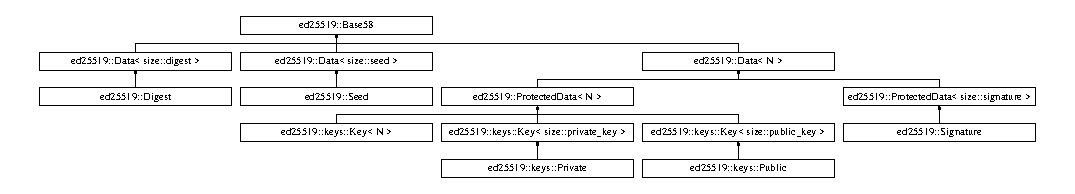
\includegraphics[height=1.278539cm]{classed25519_1_1_base58}
\end{center}
\end{figure}
\subsection*{Public Member Functions}
\begin{DoxyCompactItemize}
\item 
virtual const std\+::string \mbox{\hyperlink{classed25519_1_1_base58_a1b52a018a5215e2dcf2aa388b0fe06bf}{encode}} () const =0
\item 
virtual bool \mbox{\hyperlink{classed25519_1_1_base58_a3cb74be32923dcfb03a24b65015bee84}{decode}} (const std\+::string \&base58\+\_\+string, const \mbox{\hyperlink{namespaceed25519_a6ba572942b3c18591fc869d52a6b16e6}{Error\+Handler}} \&\mbox{\hyperlink{namespaceed25519_ac93d0b5156eaca22197055e902920bc4}{error}}=\mbox{\hyperlink{namespaceed25519_a7c7bb6ed17541162959c33ed3e3b15fb}{default\+\_\+error\+\_\+handler}})=0
\item 
virtual bool \mbox{\hyperlink{classed25519_1_1_base58_addfdb1d6d0f7e7f0cd0cf5dd2ee193bb}{validate}} () const =0
\end{DoxyCompactItemize}


\subsection{Detailed Description}
Common \mbox{\hyperlink{namespaceed25519_1_1base58}{base58}} encoding/decoding protocol 

\subsection{Member Function Documentation}
\mbox{\Hypertarget{classed25519_1_1_base58_a3cb74be32923dcfb03a24b65015bee84}\label{classed25519_1_1_base58_a3cb74be32923dcfb03a24b65015bee84}} 
\index{ed25519\+::\+Base58@{ed25519\+::\+Base58}!decode@{decode}}
\index{decode@{decode}!ed25519\+::\+Base58@{ed25519\+::\+Base58}}
\subsubsection{\texorpdfstring{decode()}{decode()}}
{\footnotesize\ttfamily virtual bool ed25519\+::\+Base58\+::decode (\begin{DoxyParamCaption}\item[{const std\+::string \&}]{base58\+\_\+string,  }\item[{const \mbox{\hyperlink{namespaceed25519_a6ba572942b3c18591fc869d52a6b16e6}{Error\+Handler}} \&}]{error = {\ttfamily \mbox{\hyperlink{namespaceed25519_a7c7bb6ed17541162959c33ed3e3b15fb}{default\+\_\+error\+\_\+handler}}} }\end{DoxyParamCaption})\hspace{0.3cm}{\ttfamily [pure virtual]}}

Decode string from \mbox{\hyperlink{namespaceed25519_1_1base58}{base58}} string


\begin{DoxyParams}{Parameters}
{\em base58\+\_\+string} & -\/ encoded string \\
\hline
{\em error} & -\/ handle error if key couldn\textquotesingle{}t ber read from string \\
\hline
\end{DoxyParams}
\begin{DoxyReturn}{Returns}
true or false 
\end{DoxyReturn}


Implemented in \mbox{\hyperlink{classed25519_1_1_data_a281d932d3c3fe7fd40ce86ea7eff559b}{ed25519\+::\+Data$<$ N $>$}}, \mbox{\hyperlink{classed25519_1_1_data_a281d932d3c3fe7fd40ce86ea7eff559b}{ed25519\+::\+Data$<$ size\+::signature $>$}}, \mbox{\hyperlink{classed25519_1_1_data_a281d932d3c3fe7fd40ce86ea7eff559b}{ed25519\+::\+Data$<$ size\+::public\+\_\+key $>$}}, \mbox{\hyperlink{classed25519_1_1_data_a281d932d3c3fe7fd40ce86ea7eff559b}{ed25519\+::\+Data$<$ size\+::private\+\_\+key $>$}}, \mbox{\hyperlink{classed25519_1_1_data_a281d932d3c3fe7fd40ce86ea7eff559b}{ed25519\+::\+Data$<$ size\+::seed $>$}}, and \mbox{\hyperlink{classed25519_1_1_data_a281d932d3c3fe7fd40ce86ea7eff559b}{ed25519\+::\+Data$<$ size\+::digest $>$}}.

\mbox{\Hypertarget{classed25519_1_1_base58_a1b52a018a5215e2dcf2aa388b0fe06bf}\label{classed25519_1_1_base58_a1b52a018a5215e2dcf2aa388b0fe06bf}} 
\index{ed25519\+::\+Base58@{ed25519\+::\+Base58}!encode@{encode}}
\index{encode@{encode}!ed25519\+::\+Base58@{ed25519\+::\+Base58}}
\subsubsection{\texorpdfstring{encode()}{encode()}}
{\footnotesize\ttfamily virtual const std\+::string ed25519\+::\+Base58\+::encode (\begin{DoxyParamCaption}{ }\end{DoxyParamCaption}) const\hspace{0.3cm}{\ttfamily [pure virtual]}}

Encode key data to \mbox{\hyperlink{namespaceed25519_1_1base58}{base58}} string \begin{DoxyReturn}{Returns}
encoded \mbox{\hyperlink{namespaceed25519_1_1base58}{base58}} string 
\end{DoxyReturn}


Implemented in \mbox{\hyperlink{classed25519_1_1_data_a2dc2e23b950a10b168d7509a63ffca53}{ed25519\+::\+Data$<$ N $>$}}, \mbox{\hyperlink{classed25519_1_1_data_a2dc2e23b950a10b168d7509a63ffca53}{ed25519\+::\+Data$<$ size\+::signature $>$}}, \mbox{\hyperlink{classed25519_1_1_data_a2dc2e23b950a10b168d7509a63ffca53}{ed25519\+::\+Data$<$ size\+::public\+\_\+key $>$}}, \mbox{\hyperlink{classed25519_1_1_data_a2dc2e23b950a10b168d7509a63ffca53}{ed25519\+::\+Data$<$ size\+::private\+\_\+key $>$}}, \mbox{\hyperlink{classed25519_1_1_data_a2dc2e23b950a10b168d7509a63ffca53}{ed25519\+::\+Data$<$ size\+::seed $>$}}, and \mbox{\hyperlink{classed25519_1_1_data_a2dc2e23b950a10b168d7509a63ffca53}{ed25519\+::\+Data$<$ size\+::digest $>$}}.

\mbox{\Hypertarget{classed25519_1_1_base58_addfdb1d6d0f7e7f0cd0cf5dd2ee193bb}\label{classed25519_1_1_base58_addfdb1d6d0f7e7f0cd0cf5dd2ee193bb}} 
\index{ed25519\+::\+Base58@{ed25519\+::\+Base58}!validate@{validate}}
\index{validate@{validate}!ed25519\+::\+Base58@{ed25519\+::\+Base58}}
\subsubsection{\texorpdfstring{validate()}{validate()}}
{\footnotesize\ttfamily virtual bool ed25519\+::\+Base58\+::validate (\begin{DoxyParamCaption}{ }\end{DoxyParamCaption}) const\hspace{0.3cm}{\ttfamily [pure virtual]}}

Validate \mbox{\hyperlink{namespaceed25519_1_1base58}{base58}} string without creating object instance 
\begin{DoxyParams}{Parameters}
{\em \mbox{\hyperlink{namespaceed25519_1_1base58}{base58}}} & string \\
\hline
\end{DoxyParams}
\begin{DoxyReturn}{Returns}
true if string is \mbox{\hyperlink{namespaceed25519_1_1base58}{base58}} encoded 
\end{DoxyReturn}


Implemented in \mbox{\hyperlink{classed25519_1_1_data_ac365c9862b45379c677449b622c74da5}{ed25519\+::\+Data$<$ N $>$}}, \mbox{\hyperlink{classed25519_1_1_data_ac365c9862b45379c677449b622c74da5}{ed25519\+::\+Data$<$ size\+::signature $>$}}, \mbox{\hyperlink{classed25519_1_1_data_ac365c9862b45379c677449b622c74da5}{ed25519\+::\+Data$<$ size\+::public\+\_\+key $>$}}, \mbox{\hyperlink{classed25519_1_1_data_ac365c9862b45379c677449b622c74da5}{ed25519\+::\+Data$<$ size\+::private\+\_\+key $>$}}, \mbox{\hyperlink{classed25519_1_1_data_ac365c9862b45379c677449b622c74da5}{ed25519\+::\+Data$<$ size\+::seed $>$}}, and \mbox{\hyperlink{classed25519_1_1_data_ac365c9862b45379c677449b622c74da5}{ed25519\+::\+Data$<$ size\+::digest $>$}}.



The documentation for this class was generated from the following file\+:\begin{DoxyCompactItemize}
\item 
/\+Users/denn/\+Development/\+Dehancer/\+Dehancer-\/\+Services/ed25519cpp/include/\mbox{\hyperlink{ed25519_8hpp}{ed25519.\+hpp}}\end{DoxyCompactItemize}

\hypertarget{classed25519_1_1_data}{}\section{ed25519\+:\+:Data$<$ N $>$ Class Template Reference}
\label{classed25519_1_1_data}\index{ed25519\+::\+Data$<$ N $>$@{ed25519\+::\+Data$<$ N $>$}}


{\ttfamily \#include $<$ed25519.\+hpp$>$}

Inheritance diagram for ed25519\+:\+:Data$<$ N $>$\+:\begin{figure}[H]
\begin{center}
\leavevmode
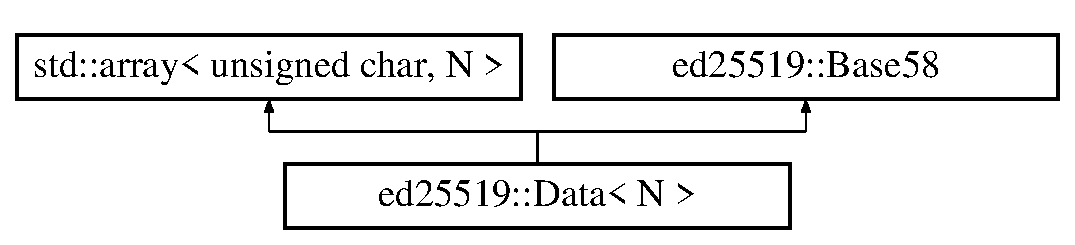
\includegraphics[height=2.000000cm]{classed25519_1_1_data}
\end{center}
\end{figure}
\subsection*{Public Member Functions}
\begin{DoxyCompactItemize}
\item 
\mbox{\hyperlink{classed25519_1_1_data_a2c637587095d6527cd4136926fb8b452}{Data}} ()
\item 
void \mbox{\hyperlink{classed25519_1_1_data_a65d5eba2b3c68f68001ef4d32645f9d9}{clean}} ()
\item 
const std\+::string \mbox{\hyperlink{classed25519_1_1_data_a2dc2e23b950a10b168d7509a63ffca53}{encode}} () const override
\item 
bool \mbox{\hyperlink{classed25519_1_1_data_a281d932d3c3fe7fd40ce86ea7eff559b}{decode}} (const std\+::string \&base58, const \mbox{\hyperlink{namespaceed25519_a6ba572942b3c18591fc869d52a6b16e6}{Error\+Handler}} \&\mbox{\hyperlink{namespaceed25519_ac93d0b5156eaca22197055e902920bc4}{error}}=\mbox{\hyperlink{namespaceed25519_a7c7bb6ed17541162959c33ed3e3b15fb}{default\+\_\+error\+\_\+handler}}) override
\item 
bool \mbox{\hyperlink{classed25519_1_1_data_ac365c9862b45379c677449b622c74da5}{validate}} () const override
\end{DoxyCompactItemize}
\subsection*{Static Public Member Functions}
\begin{DoxyCompactItemize}
\item 
static bool \mbox{\hyperlink{classed25519_1_1_data_ade9c93cb08f9d60aa45e75821ed1bcbe}{validate}} (const std\+::string \&string)
\end{DoxyCompactItemize}


\subsection{Detailed Description}
\subsubsection*{template$<$size\+\_\+t N$>$\newline
class ed25519\+::\+Data$<$ N $>$}

\mbox{\hyperlink{classed25519_1_1_base58}{Base58}} binary data structure 
\begin{DoxyTemplParams}{Template Parameters}
{\em N} & \\
\hline
\end{DoxyTemplParams}


\subsection{Constructor \& Destructor Documentation}
\mbox{\Hypertarget{classed25519_1_1_data_a2c637587095d6527cd4136926fb8b452}\label{classed25519_1_1_data_a2c637587095d6527cd4136926fb8b452}} 
\index{ed25519\+::\+Data@{ed25519\+::\+Data}!Data@{Data}}
\index{Data@{Data}!ed25519\+::\+Data@{ed25519\+::\+Data}}
\subsubsection{\texorpdfstring{Data()}{Data()}}
{\footnotesize\ttfamily template$<$size\+\_\+t N$>$ \\
\mbox{\hyperlink{classed25519_1_1_data}{ed25519\+::\+Data}}$<$ N $>$\+::\mbox{\hyperlink{classed25519_1_1_data}{Data}} (\begin{DoxyParamCaption}{ }\end{DoxyParamCaption})\hspace{0.3cm}{\ttfamily [inline]}}



\subsection{Member Function Documentation}
\mbox{\Hypertarget{classed25519_1_1_data_a65d5eba2b3c68f68001ef4d32645f9d9}\label{classed25519_1_1_data_a65d5eba2b3c68f68001ef4d32645f9d9}} 
\index{ed25519\+::\+Data@{ed25519\+::\+Data}!clean@{clean}}
\index{clean@{clean}!ed25519\+::\+Data@{ed25519\+::\+Data}}
\subsubsection{\texorpdfstring{clean()}{clean()}}
{\footnotesize\ttfamily template$<$size\+\_\+t N$>$ \\
void \mbox{\hyperlink{classed25519_1_1_data}{ed25519\+::\+Data}}$<$ N $>$\+::clean (\begin{DoxyParamCaption}{ }\end{DoxyParamCaption})\hspace{0.3cm}{\ttfamily [inline]}}

Clean data memory \mbox{\Hypertarget{classed25519_1_1_data_a281d932d3c3fe7fd40ce86ea7eff559b}\label{classed25519_1_1_data_a281d932d3c3fe7fd40ce86ea7eff559b}} 
\index{ed25519\+::\+Data@{ed25519\+::\+Data}!decode@{decode}}
\index{decode@{decode}!ed25519\+::\+Data@{ed25519\+::\+Data}}
\subsubsection{\texorpdfstring{decode()}{decode()}}
{\footnotesize\ttfamily template$<$size\+\_\+t N$>$ \\
bool \mbox{\hyperlink{classed25519_1_1_data}{ed25519\+::\+Data}}$<$ N $>$\+::decode (\begin{DoxyParamCaption}\item[{const std\+::string \&}]{base58,  }\item[{const \mbox{\hyperlink{namespaceed25519_a6ba572942b3c18591fc869d52a6b16e6}{Error\+Handler}} \&}]{error = {\ttfamily \mbox{\hyperlink{namespaceed25519_a7c7bb6ed17541162959c33ed3e3b15fb}{default\+\_\+error\+\_\+handler}}} }\end{DoxyParamCaption})\hspace{0.3cm}{\ttfamily [inline]}, {\ttfamily [override]}, {\ttfamily [virtual]}}

Decode \mbox{\hyperlink{namespaceed25519_1_1base58}{base58}} encoded string to binary represenation 
\begin{DoxyParams}{Parameters}
{\em \mbox{\hyperlink{namespaceed25519_1_1base58}{base58}}} & encoded string \\
\hline
{\em error} & -\/ error handler \\
\hline
\end{DoxyParams}
\begin{DoxyReturn}{Returns}
false if decoding is failed 
\end{DoxyReturn}


Implements \mbox{\hyperlink{classed25519_1_1_base58_a3cb74be32923dcfb03a24b65015bee84}{ed25519\+::\+Base58}}.

\mbox{\Hypertarget{classed25519_1_1_data_a2dc2e23b950a10b168d7509a63ffca53}\label{classed25519_1_1_data_a2dc2e23b950a10b168d7509a63ffca53}} 
\index{ed25519\+::\+Data@{ed25519\+::\+Data}!encode@{encode}}
\index{encode@{encode}!ed25519\+::\+Data@{ed25519\+::\+Data}}
\subsubsection{\texorpdfstring{encode()}{encode()}}
{\footnotesize\ttfamily template$<$size\+\_\+t N$>$ \\
const std\+::string \mbox{\hyperlink{classed25519_1_1_data}{ed25519\+::\+Data}}$<$ N $>$\+::encode (\begin{DoxyParamCaption}{ }\end{DoxyParamCaption}) const\hspace{0.3cm}{\ttfamily [inline]}, {\ttfamily [override]}, {\ttfamily [virtual]}}

Encode from binary to \mbox{\hyperlink{namespaceed25519_1_1base58}{base58}} encoded string \begin{DoxyReturn}{Returns}
encoded string 
\end{DoxyReturn}


Implements \mbox{\hyperlink{classed25519_1_1_base58_a1b52a018a5215e2dcf2aa388b0fe06bf}{ed25519\+::\+Base58}}.

\mbox{\Hypertarget{classed25519_1_1_data_ac365c9862b45379c677449b622c74da5}\label{classed25519_1_1_data_ac365c9862b45379c677449b622c74da5}} 
\index{ed25519\+::\+Data@{ed25519\+::\+Data}!validate@{validate}}
\index{validate@{validate}!ed25519\+::\+Data@{ed25519\+::\+Data}}
\subsubsection{\texorpdfstring{validate()}{validate()}\hspace{0.1cm}{\footnotesize\ttfamily [1/2]}}
{\footnotesize\ttfamily template$<$size\+\_\+t N$>$ \\
bool \mbox{\hyperlink{classed25519_1_1_data}{ed25519\+::\+Data}}$<$ N $>$\+::validate (\begin{DoxyParamCaption}{ }\end{DoxyParamCaption}) const\hspace{0.3cm}{\ttfamily [inline]}, {\ttfamily [override]}, {\ttfamily [virtual]}}

Validate \mbox{\hyperlink{namespaceed25519_1_1base58}{base58}} string without creating object instance 
\begin{DoxyParams}{Parameters}
{\em \mbox{\hyperlink{namespaceed25519_1_1base58}{base58}}} & string \\
\hline
\end{DoxyParams}
\begin{DoxyReturn}{Returns}
true if string is \mbox{\hyperlink{namespaceed25519_1_1base58}{base58}} encoded 
\end{DoxyReturn}


Implements \mbox{\hyperlink{classed25519_1_1_base58_addfdb1d6d0f7e7f0cd0cf5dd2ee193bb}{ed25519\+::\+Base58}}.

\mbox{\Hypertarget{classed25519_1_1_data_ade9c93cb08f9d60aa45e75821ed1bcbe}\label{classed25519_1_1_data_ade9c93cb08f9d60aa45e75821ed1bcbe}} 
\index{ed25519\+::\+Data@{ed25519\+::\+Data}!validate@{validate}}
\index{validate@{validate}!ed25519\+::\+Data@{ed25519\+::\+Data}}
\subsubsection{\texorpdfstring{validate()}{validate()}\hspace{0.1cm}{\footnotesize\ttfamily [2/2]}}
{\footnotesize\ttfamily template$<$size\+\_\+t N$>$ \\
static bool \mbox{\hyperlink{classed25519_1_1_data}{ed25519\+::\+Data}}$<$ N $>$\+::validate (\begin{DoxyParamCaption}\item[{const std\+::string \&}]{string }\end{DoxyParamCaption})\hspace{0.3cm}{\ttfamily [inline]}, {\ttfamily [static]}}

Validate string before create encoded data. 
\begin{DoxyParams}{Parameters}
{\em string} & \\
\hline
\end{DoxyParams}
\begin{DoxyReturn}{Returns}
validation result 
\end{DoxyReturn}


The documentation for this class was generated from the following file\+:\begin{DoxyCompactItemize}
\item 
/\+Users/denn/\+Development/\+Dehancer/\+Dehancer-\/\+Services/ed25519cpp/include/\mbox{\hyperlink{ed25519_8hpp}{ed25519.\+hpp}}\end{DoxyCompactItemize}

\hypertarget{structed25519_1_1_digest}{}\section{ed25519\+:\+:Digest Struct Reference}
\label{structed25519_1_1_digest}\index{ed25519\+::\+Digest@{ed25519\+::\+Digest}}


{\ttfamily \#include $<$ed25519.\+hpp$>$}

Inheritance diagram for ed25519\+:\+:Digest\+:\begin{figure}[H]
\begin{center}
\leavevmode
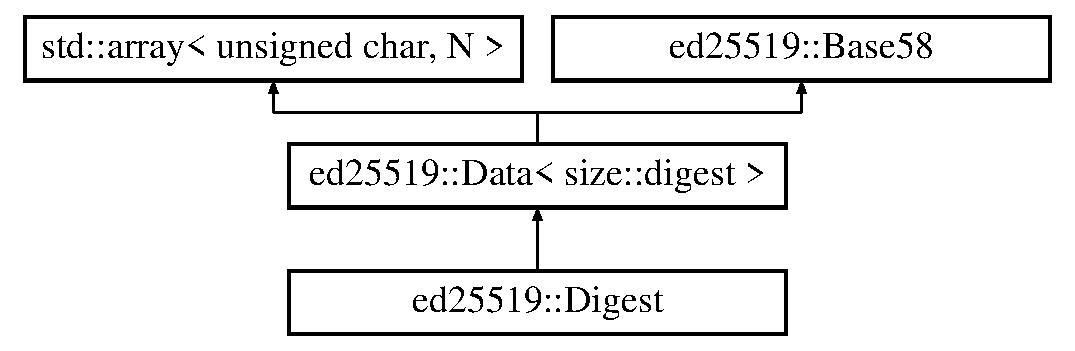
\includegraphics[height=3.000000cm]{structed25519_1_1_digest}
\end{center}
\end{figure}
\subsection*{Additional Inherited Members}


\subsection{Detailed Description}
\mbox{\hyperlink{structed25519_1_1_digest}{Digest}} hash class 

The documentation for this struct was generated from the following file\+:\begin{DoxyCompactItemize}
\item 
/\+Users/denn/\+Development/\+Dehancer/\+Dehancer-\/\+Services/ed25519cpp/include/\mbox{\hyperlink{ed25519_8hpp}{ed25519.\+hpp}}\end{DoxyCompactItemize}

\hypertarget{classed25519_1_1error__category}{}\section{ed25519\+::error\+\_\+category Class Reference}
\label{classed25519_1_1error__category}\index{ed25519::error\_category@{ed25519::error\_category}}


{\ttfamily \#include $<$ed25519.\+hpp$>$}

Inheritance diagram for ed25519\+::error\+\_\+category\+:\begin{figure}[H]
\begin{center}
\leavevmode
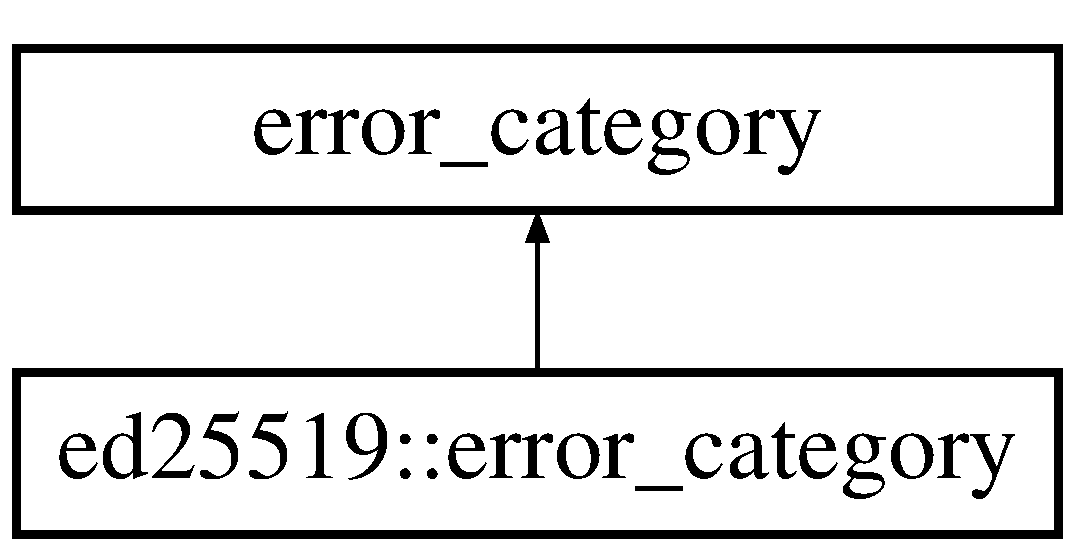
\includegraphics[height=2.000000cm]{classed25519_1_1error__category}
\end{center}
\end{figure}
\subsection*{Public Member Functions}
\begin{DoxyCompactItemize}
\item 
\mbox{\hyperlink{classed25519_1_1error__category_a6150d658628877349385868102b0b9af}{error\+\_\+category}} (const std\+::string \&\mbox{\hyperlink{classed25519_1_1error__category_a202bf6ba84147b563f630c8f52c723ef}{message}})
\item 
\mbox{\hyperlink{classed25519_1_1error__category_a4fe3061ad89abff2d326dacbae9cee7d}{error\+\_\+category}} ()
\item 
const char $\ast$ \mbox{\hyperlink{classed25519_1_1error__category_a4bdacefbd1473eea02c945905230b6ce}{name}} () const noexcept override
\item 
std\+::string \mbox{\hyperlink{classed25519_1_1error__category_a202bf6ba84147b563f630c8f52c723ef}{message}} (int ev) const override
\end{DoxyCompactItemize}


\subsection{Constructor \& Destructor Documentation}
\mbox{\Hypertarget{classed25519_1_1error__category_a6150d658628877349385868102b0b9af}\label{classed25519_1_1error__category_a6150d658628877349385868102b0b9af}} 
\index{ed25519::error\_category@{ed25519::error\_category}!error\_category@{error\_category}}
\index{error\_category@{error\_category}!ed25519::error\_category@{ed25519::error\_category}}
\subsubsection{\texorpdfstring{error\_category()}{error\_category()}\hspace{0.1cm}{\footnotesize\ttfamily [1/2]}}
{\footnotesize\ttfamily ed25519\+::error\+\_\+category\+::error\+\_\+category (\begin{DoxyParamCaption}\item[{const std\+::string \&}]{message }\end{DoxyParamCaption})}

\mbox{\Hypertarget{classed25519_1_1error__category_a4fe3061ad89abff2d326dacbae9cee7d}\label{classed25519_1_1error__category_a4fe3061ad89abff2d326dacbae9cee7d}} 
\index{ed25519::error\_category@{ed25519::error\_category}!error\_category@{error\_category}}
\index{error\_category@{error\_category}!ed25519::error\_category@{ed25519::error\_category}}
\subsubsection{\texorpdfstring{error\_category()}{error\_category()}\hspace{0.1cm}{\footnotesize\ttfamily [2/2]}}
{\footnotesize\ttfamily ed25519\+::error\+\_\+category\+::error\+\_\+category (\begin{DoxyParamCaption}{ }\end{DoxyParamCaption})\hspace{0.3cm}{\ttfamily [inline]}}



\subsection{Member Function Documentation}
\mbox{\Hypertarget{classed25519_1_1error__category_a202bf6ba84147b563f630c8f52c723ef}\label{classed25519_1_1error__category_a202bf6ba84147b563f630c8f52c723ef}} 
\index{ed25519::error\_category@{ed25519::error\_category}!message@{message}}
\index{message@{message}!ed25519::error\_category@{ed25519::error\_category}}
\subsubsection{\texorpdfstring{message()}{message()}}
{\footnotesize\ttfamily std\+::string ed25519\+::error\+\_\+category\+::message (\begin{DoxyParamCaption}\item[{int}]{ev }\end{DoxyParamCaption}) const\hspace{0.3cm}{\ttfamily [override]}}

\mbox{\Hypertarget{classed25519_1_1error__category_a4bdacefbd1473eea02c945905230b6ce}\label{classed25519_1_1error__category_a4bdacefbd1473eea02c945905230b6ce}} 
\index{ed25519::error\_category@{ed25519::error\_category}!name@{name}}
\index{name@{name}!ed25519::error\_category@{ed25519::error\_category}}
\subsubsection{\texorpdfstring{name()}{name()}}
{\footnotesize\ttfamily const char$\ast$ ed25519\+::error\+\_\+category\+::name (\begin{DoxyParamCaption}{ }\end{DoxyParamCaption}) const\hspace{0.3cm}{\ttfamily [override]}, {\ttfamily [noexcept]}}



The documentation for this class was generated from the following file\+:\begin{DoxyCompactItemize}
\item 
/\+Users/denn/\+Development/\+Dehancer/\+Dehancer-\/\+Services/ed25519cpp/include/\mbox{\hyperlink{ed25519_8hpp}{ed25519.\+hpp}}\end{DoxyCompactItemize}

\hypertarget{classed25519_1_1keys_1_1_pair}{}\section{ed25519\+:\+:keys\+:\+:Pair Class Reference}
\label{classed25519_1_1keys_1_1_pair}\index{ed25519\+::keys\+::\+Pair@{ed25519\+::keys\+::\+Pair}}


{\ttfamily \#include $<$ed25519.\+hpp$>$}

\subsection*{Public Member Functions}
\begin{DoxyCompactItemize}
\item 
const \mbox{\hyperlink{classed25519_1_1keys_1_1_public}{Public}} \& \mbox{\hyperlink{classed25519_1_1keys_1_1_pair_aad6c01fdb3b75ce2b05e51dbc833ac72}{get\+\_\+public\+\_\+key}} () const
\item 
const \mbox{\hyperlink{classed25519_1_1keys_1_1_private}{Private}} \& \mbox{\hyperlink{classed25519_1_1keys_1_1_pair_add9c9587c53dff8b1d5bc69a7a97f837}{get\+\_\+private\+\_\+key}} () const
\item 
void \mbox{\hyperlink{classed25519_1_1keys_1_1_pair_ae803e41096e0f6edb030e48713515aa2}{clean}} ()
\item 
bool \mbox{\hyperlink{classed25519_1_1keys_1_1_pair_a36436b3c74b785a8ef2a712525761044}{validate}} ()
\item 
std\+::unique\+\_\+ptr$<$ \mbox{\hyperlink{classed25519_1_1_signature}{Signature}} $>$ \mbox{\hyperlink{classed25519_1_1keys_1_1_pair_ad92702362f23ad3d55e2d226e056c742}{sign}} (const std\+::vector$<$ unsigned char $>$ \&message)
\item 
std\+::unique\+\_\+ptr$<$ \mbox{\hyperlink{classed25519_1_1_signature}{Signature}} $>$ \mbox{\hyperlink{classed25519_1_1keys_1_1_pair_a1c53cc9aff7f89d8cefc27eb99d42f8d}{sign}} (const std\+::string \&message)
\item 
std\+::unique\+\_\+ptr$<$ \mbox{\hyperlink{classed25519_1_1_signature}{Signature}} $>$ \mbox{\hyperlink{classed25519_1_1keys_1_1_pair_ac1c7387192283f87fc16acf53eb9c313}{sign}} (const \mbox{\hyperlink{structed25519_1_1_digest}{Digest}} \&digest)
\item 
\mbox{\hyperlink{classed25519_1_1keys_1_1_pair_a23edc59bc943684eadbdae8ffd6c8a42}{$\sim$\+Pair}} ()
\end{DoxyCompactItemize}
\subsection*{Static Public Member Functions}
\begin{DoxyCompactItemize}
\item 
static std\+::optional$<$ \mbox{\hyperlink{classed25519_1_1keys_1_1_pair}{Pair}} $>$ \mbox{\hyperlink{classed25519_1_1keys_1_1_pair_a56deb8f1bf6d1a51313abebd5a41d6fc}{Random}} ()
\item 
static std\+::optional$<$ \mbox{\hyperlink{classed25519_1_1keys_1_1_pair}{Pair}} $>$ \mbox{\hyperlink{classed25519_1_1keys_1_1_pair_aa4b34f7823cbba1e4243b9fbf2745e1e}{From\+Private\+Key}} (const std\+::string \&private\+Key, const \mbox{\hyperlink{namespaceed25519_a6ba572942b3c18591fc869d52a6b16e6}{Error\+Handler}} \&\mbox{\hyperlink{namespaceed25519_ac93d0b5156eaca22197055e902920bc4}{error}}=\mbox{\hyperlink{namespaceed25519_a7c7bb6ed17541162959c33ed3e3b15fb}{default\+\_\+error\+\_\+handler}})
\item 
static std\+::optional$<$ \mbox{\hyperlink{classed25519_1_1keys_1_1_pair}{Pair}} $>$ \mbox{\hyperlink{classed25519_1_1keys_1_1_pair_a3d7457b834d7e8091a61272f20132d01}{With\+Secret}} (const std\+::string \&phrase, const \mbox{\hyperlink{namespaceed25519_a6ba572942b3c18591fc869d52a6b16e6}{Error\+Handler}} \&\mbox{\hyperlink{namespaceed25519_ac93d0b5156eaca22197055e902920bc4}{error}}=\mbox{\hyperlink{namespaceed25519_a7c7bb6ed17541162959c33ed3e3b15fb}{default\+\_\+error\+\_\+handler}})
\end{DoxyCompactItemize}


\subsection{Detailed Description}
\mbox{\hyperlink{classed25519_1_1keys_1_1_pair}{Pair}} key representation 

\subsection{Constructor \& Destructor Documentation}
\mbox{\Hypertarget{classed25519_1_1keys_1_1_pair_a23edc59bc943684eadbdae8ffd6c8a42}\label{classed25519_1_1keys_1_1_pair_a23edc59bc943684eadbdae8ffd6c8a42}} 
\index{ed25519\+::keys\+::\+Pair@{ed25519\+::keys\+::\+Pair}!````~Pair@{$\sim$\+Pair}}
\index{````~Pair@{$\sim$\+Pair}!ed25519\+::keys\+::\+Pair@{ed25519\+::keys\+::\+Pair}}
\subsubsection{\texorpdfstring{$\sim$\+Pair()}{~Pair()}}
{\footnotesize\ttfamily ed25519\+::keys\+::\+Pair\+::$\sim$\+Pair (\begin{DoxyParamCaption}{ }\end{DoxyParamCaption})\hspace{0.3cm}{\ttfamily [inline]}}



\subsection{Member Function Documentation}
\mbox{\Hypertarget{classed25519_1_1keys_1_1_pair_ae803e41096e0f6edb030e48713515aa2}\label{classed25519_1_1keys_1_1_pair_ae803e41096e0f6edb030e48713515aa2}} 
\index{ed25519\+::keys\+::\+Pair@{ed25519\+::keys\+::\+Pair}!clean@{clean}}
\index{clean@{clean}!ed25519\+::keys\+::\+Pair@{ed25519\+::keys\+::\+Pair}}
\subsubsection{\texorpdfstring{clean()}{clean()}}
{\footnotesize\ttfamily void ed25519\+::keys\+::\+Pair\+::clean (\begin{DoxyParamCaption}{ }\end{DoxyParamCaption})}

Clean pair \mbox{\Hypertarget{classed25519_1_1keys_1_1_pair_aa4b34f7823cbba1e4243b9fbf2745e1e}\label{classed25519_1_1keys_1_1_pair_aa4b34f7823cbba1e4243b9fbf2745e1e}} 
\index{ed25519\+::keys\+::\+Pair@{ed25519\+::keys\+::\+Pair}!From\+Private\+Key@{From\+Private\+Key}}
\index{From\+Private\+Key@{From\+Private\+Key}!ed25519\+::keys\+::\+Pair@{ed25519\+::keys\+::\+Pair}}
\subsubsection{\texorpdfstring{From\+Private\+Key()}{FromPrivateKey()}}
{\footnotesize\ttfamily static std\+::optional$<$\mbox{\hyperlink{classed25519_1_1keys_1_1_pair}{Pair}}$>$ ed25519\+::keys\+::\+Pair\+::\+From\+Private\+Key (\begin{DoxyParamCaption}\item[{const std\+::string \&}]{private\+Key,  }\item[{const \mbox{\hyperlink{namespaceed25519_a6ba572942b3c18591fc869d52a6b16e6}{Error\+Handler}} \&}]{error = {\ttfamily \mbox{\hyperlink{namespaceed25519_a7c7bb6ed17541162959c33ed3e3b15fb}{default\+\_\+error\+\_\+handler}}} }\end{DoxyParamCaption})\hspace{0.3cm}{\ttfamily [static]}}

Create random pair \begin{DoxyReturn}{Returns}
always exists private key 
\end{DoxyReturn}
\mbox{\Hypertarget{classed25519_1_1keys_1_1_pair_add9c9587c53dff8b1d5bc69a7a97f837}\label{classed25519_1_1keys_1_1_pair_add9c9587c53dff8b1d5bc69a7a97f837}} 
\index{ed25519\+::keys\+::\+Pair@{ed25519\+::keys\+::\+Pair}!get\+\_\+private\+\_\+key@{get\+\_\+private\+\_\+key}}
\index{get\+\_\+private\+\_\+key@{get\+\_\+private\+\_\+key}!ed25519\+::keys\+::\+Pair@{ed25519\+::keys\+::\+Pair}}
\subsubsection{\texorpdfstring{get\+\_\+private\+\_\+key()}{get\_private\_key()}}
{\footnotesize\ttfamily const \mbox{\hyperlink{classed25519_1_1keys_1_1_private}{Private}}\& ed25519\+::keys\+::\+Pair\+::get\+\_\+private\+\_\+key (\begin{DoxyParamCaption}{ }\end{DoxyParamCaption}) const\hspace{0.3cm}{\ttfamily [inline]}}

\mbox{\Hypertarget{classed25519_1_1keys_1_1_pair_aad6c01fdb3b75ce2b05e51dbc833ac72}\label{classed25519_1_1keys_1_1_pair_aad6c01fdb3b75ce2b05e51dbc833ac72}} 
\index{ed25519\+::keys\+::\+Pair@{ed25519\+::keys\+::\+Pair}!get\+\_\+public\+\_\+key@{get\+\_\+public\+\_\+key}}
\index{get\+\_\+public\+\_\+key@{get\+\_\+public\+\_\+key}!ed25519\+::keys\+::\+Pair@{ed25519\+::keys\+::\+Pair}}
\subsubsection{\texorpdfstring{get\+\_\+public\+\_\+key()}{get\_public\_key()}}
{\footnotesize\ttfamily const \mbox{\hyperlink{classed25519_1_1keys_1_1_public}{Public}}\& ed25519\+::keys\+::\+Pair\+::get\+\_\+public\+\_\+key (\begin{DoxyParamCaption}{ }\end{DoxyParamCaption}) const\hspace{0.3cm}{\ttfamily [inline]}}

Get paired public key for the private \begin{DoxyReturn}{Returns}
copy of public key 
\end{DoxyReturn}
\mbox{\Hypertarget{classed25519_1_1keys_1_1_pair_a56deb8f1bf6d1a51313abebd5a41d6fc}\label{classed25519_1_1keys_1_1_pair_a56deb8f1bf6d1a51313abebd5a41d6fc}} 
\index{ed25519\+::keys\+::\+Pair@{ed25519\+::keys\+::\+Pair}!Random@{Random}}
\index{Random@{Random}!ed25519\+::keys\+::\+Pair@{ed25519\+::keys\+::\+Pair}}
\subsubsection{\texorpdfstring{Random()}{Random()}}
{\footnotesize\ttfamily static std\+::optional$<$\mbox{\hyperlink{classed25519_1_1keys_1_1_pair}{Pair}}$>$ ed25519\+::keys\+::\+Pair\+::\+Random (\begin{DoxyParamCaption}{ }\end{DoxyParamCaption})\hspace{0.3cm}{\ttfamily [static]}}

Create random pair \begin{DoxyReturn}{Returns}
always exists private key 
\end{DoxyReturn}
\mbox{\Hypertarget{classed25519_1_1keys_1_1_pair_ad92702362f23ad3d55e2d226e056c742}\label{classed25519_1_1keys_1_1_pair_ad92702362f23ad3d55e2d226e056c742}} 
\index{ed25519\+::keys\+::\+Pair@{ed25519\+::keys\+::\+Pair}!sign@{sign}}
\index{sign@{sign}!ed25519\+::keys\+::\+Pair@{ed25519\+::keys\+::\+Pair}}
\subsubsection{\texorpdfstring{sign()}{sign()}\hspace{0.1cm}{\footnotesize\ttfamily [1/3]}}
{\footnotesize\ttfamily std\+::unique\+\_\+ptr$<$\mbox{\hyperlink{classed25519_1_1_signature}{Signature}}$>$ ed25519\+::keys\+::\+Pair\+::sign (\begin{DoxyParamCaption}\item[{const std\+::vector$<$ unsigned char $>$ \&}]{message }\end{DoxyParamCaption})}

Sign a message 
\begin{DoxyParams}{Parameters}
{\em message} & data \\
\hline
\end{DoxyParams}
\begin{DoxyReturn}{Returns}
signature hash 
\end{DoxyReturn}
\mbox{\Hypertarget{classed25519_1_1keys_1_1_pair_a1c53cc9aff7f89d8cefc27eb99d42f8d}\label{classed25519_1_1keys_1_1_pair_a1c53cc9aff7f89d8cefc27eb99d42f8d}} 
\index{ed25519\+::keys\+::\+Pair@{ed25519\+::keys\+::\+Pair}!sign@{sign}}
\index{sign@{sign}!ed25519\+::keys\+::\+Pair@{ed25519\+::keys\+::\+Pair}}
\subsubsection{\texorpdfstring{sign()}{sign()}\hspace{0.1cm}{\footnotesize\ttfamily [2/3]}}
{\footnotesize\ttfamily std\+::unique\+\_\+ptr$<$\mbox{\hyperlink{classed25519_1_1_signature}{Signature}}$>$ ed25519\+::keys\+::\+Pair\+::sign (\begin{DoxyParamCaption}\item[{const std\+::string \&}]{message }\end{DoxyParamCaption})}

Sign a message 
\begin{DoxyParams}{Parameters}
{\em message} & string \\
\hline
\end{DoxyParams}
\begin{DoxyReturn}{Returns}
signature hash 
\end{DoxyReturn}
\mbox{\Hypertarget{classed25519_1_1keys_1_1_pair_ac1c7387192283f87fc16acf53eb9c313}\label{classed25519_1_1keys_1_1_pair_ac1c7387192283f87fc16acf53eb9c313}} 
\index{ed25519\+::keys\+::\+Pair@{ed25519\+::keys\+::\+Pair}!sign@{sign}}
\index{sign@{sign}!ed25519\+::keys\+::\+Pair@{ed25519\+::keys\+::\+Pair}}
\subsubsection{\texorpdfstring{sign()}{sign()}\hspace{0.1cm}{\footnotesize\ttfamily [3/3]}}
{\footnotesize\ttfamily std\+::unique\+\_\+ptr$<$\mbox{\hyperlink{classed25519_1_1_signature}{Signature}}$>$ ed25519\+::keys\+::\+Pair\+::sign (\begin{DoxyParamCaption}\item[{const \mbox{\hyperlink{structed25519_1_1_digest}{Digest}} \&}]{digest }\end{DoxyParamCaption})}

Sign a digest 
\begin{DoxyParams}{Parameters}
{\em digest} & data \\
\hline
\end{DoxyParams}
\begin{DoxyReturn}{Returns}
signature hash 
\end{DoxyReturn}
\mbox{\Hypertarget{classed25519_1_1keys_1_1_pair_a36436b3c74b785a8ef2a712525761044}\label{classed25519_1_1keys_1_1_pair_a36436b3c74b785a8ef2a712525761044}} 
\index{ed25519\+::keys\+::\+Pair@{ed25519\+::keys\+::\+Pair}!validate@{validate}}
\index{validate@{validate}!ed25519\+::keys\+::\+Pair@{ed25519\+::keys\+::\+Pair}}
\subsubsection{\texorpdfstring{validate()}{validate()}}
{\footnotesize\ttfamily bool ed25519\+::keys\+::\+Pair\+::validate (\begin{DoxyParamCaption}{ }\end{DoxyParamCaption})}

Vlidate pair \begin{DoxyReturn}{Returns}
validation result 
\end{DoxyReturn}
\mbox{\Hypertarget{classed25519_1_1keys_1_1_pair_a3d7457b834d7e8091a61272f20132d01}\label{classed25519_1_1keys_1_1_pair_a3d7457b834d7e8091a61272f20132d01}} 
\index{ed25519\+::keys\+::\+Pair@{ed25519\+::keys\+::\+Pair}!With\+Secret@{With\+Secret}}
\index{With\+Secret@{With\+Secret}!ed25519\+::keys\+::\+Pair@{ed25519\+::keys\+::\+Pair}}
\subsubsection{\texorpdfstring{With\+Secret()}{WithSecret()}}
{\footnotesize\ttfamily static std\+::optional$<$\mbox{\hyperlink{classed25519_1_1keys_1_1_pair}{Pair}}$>$ ed25519\+::keys\+::\+Pair\+::\+With\+Secret (\begin{DoxyParamCaption}\item[{const std\+::string \&}]{phrase,  }\item[{const \mbox{\hyperlink{namespaceed25519_a6ba572942b3c18591fc869d52a6b16e6}{Error\+Handler}} \&}]{error = {\ttfamily \mbox{\hyperlink{namespaceed25519_a7c7bb6ed17541162959c33ed3e3b15fb}{default\+\_\+error\+\_\+handler}}} }\end{DoxyParamCaption})\hspace{0.3cm}{\ttfamily [static]}}

Optional constructor from secret phrase 
\begin{DoxyParams}{Parameters}
{\em phrase} & \\
\hline
{\em error} & \\
\hline
\end{DoxyParams}
\begin{DoxyReturn}{Returns}
nullopt or private key 
\end{DoxyReturn}


The documentation for this class was generated from the following file\+:\begin{DoxyCompactItemize}
\item 
/\+Users/denn/\+Development/\+Dehancer/\+Dehancer-\/\+Services/ed25519cpp/include/\mbox{\hyperlink{ed25519_8hpp}{ed25519.\+hpp}}\end{DoxyCompactItemize}

\hypertarget{classed25519_1_1keys_1_1_private}{}\section{ed25519\+:\+:keys\+:\+:Private Class Reference}
\label{classed25519_1_1keys_1_1_private}\index{ed25519\+::keys\+::\+Private@{ed25519\+::keys\+::\+Private}}


{\ttfamily \#include $<$ed25519.\+hpp$>$}

Inheritance diagram for ed25519\+:\+:keys\+:\+:Private\+:\begin{figure}[H]
\begin{center}
\leavevmode
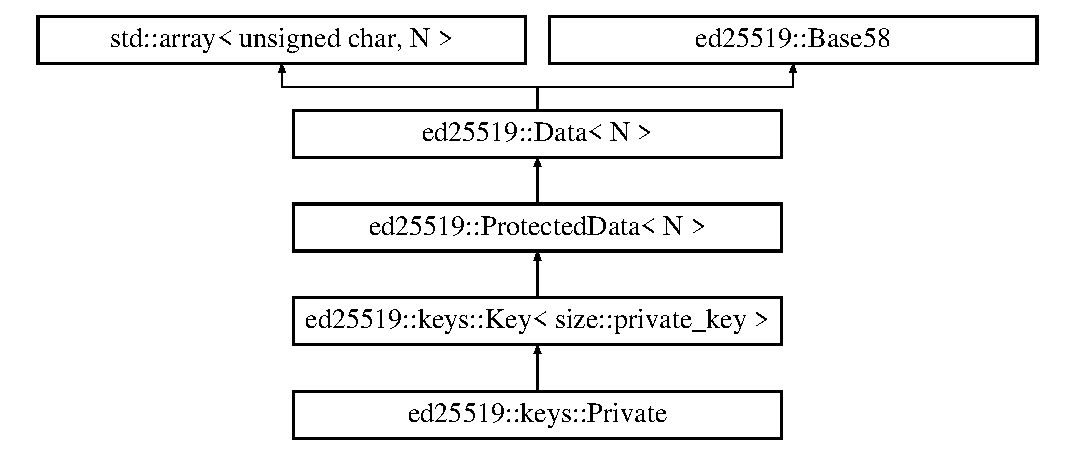
\includegraphics[height=5.000000cm]{classed25519_1_1keys_1_1_private}
\end{center}
\end{figure}
\subsection*{Friends}
\begin{DoxyCompactItemize}
\item 
class \mbox{\hyperlink{classed25519_1_1keys_1_1_private_ad89670fe663c8c8526b69b1bc6a87c19}{keys\+::\+Pair}}
\end{DoxyCompactItemize}
\subsection*{Additional Inherited Members}


\subsection{Detailed Description}
\mbox{\hyperlink{classed25519_1_1keys_1_1_private}{Private}} key representation 

\subsection{Friends And Related Function Documentation}
\mbox{\Hypertarget{classed25519_1_1keys_1_1_private_ad89670fe663c8c8526b69b1bc6a87c19}\label{classed25519_1_1keys_1_1_private_ad89670fe663c8c8526b69b1bc6a87c19}} 
\index{ed25519\+::keys\+::\+Private@{ed25519\+::keys\+::\+Private}!keys\+::\+Pair@{keys\+::\+Pair}}
\index{keys\+::\+Pair@{keys\+::\+Pair}!ed25519\+::keys\+::\+Private@{ed25519\+::keys\+::\+Private}}
\subsubsection{\texorpdfstring{keys\+::\+Pair}{keys::Pair}}
{\footnotesize\ttfamily friend class \mbox{\hyperlink{classed25519_1_1keys_1_1_pair}{keys\+::\+Pair}}\hspace{0.3cm}{\ttfamily [friend]}}



The documentation for this class was generated from the following file\+:\begin{DoxyCompactItemize}
\item 
/\+Users/denn/\+Development/\+Dehancer/\+Dehancer-\/\+Services/ed25519cpp/include/\mbox{\hyperlink{ed25519_8hpp}{ed25519.\+hpp}}\end{DoxyCompactItemize}

\hypertarget{classed25519_1_1keys_1_1_public}{}\section{ed25519\+::keys\+::Public Class Reference}
\label{classed25519_1_1keys_1_1_public}\index{ed25519::keys::Public@{ed25519::keys::Public}}


{\ttfamily \#include $<$ed25519.\+hpp$>$}

Inheritance diagram for ed25519\+::keys\+::Public\+:\begin{figure}[H]
\begin{center}
\leavevmode
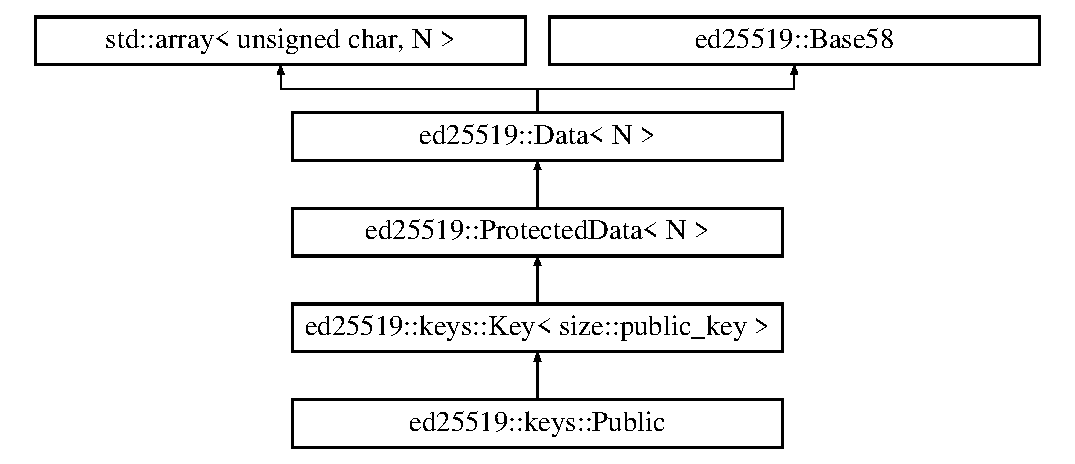
\includegraphics[height=5.000000cm]{classed25519_1_1keys_1_1_public}
\end{center}
\end{figure}
\subsection*{Static Public Member Functions}
\begin{DoxyCompactItemize}
\item 
static std\+::optional$<$ \mbox{\hyperlink{classed25519_1_1keys_1_1_public}{Public}} $>$ \mbox{\hyperlink{classed25519_1_1keys_1_1_public_af8a468caa9cc98160b65ec072f949e97}{Decode}} (const std\+::string \&base58, const \mbox{\hyperlink{namespaceed25519_a6ba572942b3c18591fc869d52a6b16e6}{Error\+Handler}} \&\mbox{\hyperlink{namespaceed25519_ac93d0b5156eaca22197055e902920bc4}{error}}=\mbox{\hyperlink{namespaceed25519_a7c7bb6ed17541162959c33ed3e3b15fb}{default\+\_\+error\+\_\+handler}})
\end{DoxyCompactItemize}
\subsection*{Additional Inherited Members}


\subsection{Detailed Description}
\mbox{\hyperlink{classed25519_1_1keys_1_1_public}{Public}} key representaion 

\subsection{Member Function Documentation}
\mbox{\Hypertarget{classed25519_1_1keys_1_1_public_af8a468caa9cc98160b65ec072f949e97}\label{classed25519_1_1keys_1_1_public_af8a468caa9cc98160b65ec072f949e97}} 
\index{ed25519::keys::Public@{ed25519::keys::Public}!Decode@{Decode}}
\index{Decode@{Decode}!ed25519::keys::Public@{ed25519::keys::Public}}
\subsubsection{\texorpdfstring{Decode()}{Decode()}}
{\footnotesize\ttfamily static std\+::optional$<$\mbox{\hyperlink{classed25519_1_1keys_1_1_public}{Public}}$>$ ed25519\+::keys\+::\+Public\+::\+Decode (\begin{DoxyParamCaption}\item[{const std\+::string \&}]{base58,  }\item[{const \mbox{\hyperlink{namespaceed25519_a6ba572942b3c18591fc869d52a6b16e6}{Error\+Handler}} \&}]{error = {\ttfamily \mbox{\hyperlink{namespaceed25519_a7c7bb6ed17541162959c33ed3e3b15fb}{default\+\_\+error\+\_\+handler}}} }\end{DoxyParamCaption})\hspace{0.3cm}{\ttfamily [static]}}



The documentation for this class was generated from the following file\+:\begin{DoxyCompactItemize}
\item 
/\+Users/denn/\+Development/\+Dehancer/\+Dehancer-\/\+Services/ed25519cpp/include/\mbox{\hyperlink{ed25519_8hpp}{ed25519.\+hpp}}\end{DoxyCompactItemize}

\hypertarget{classed25519_1_1keys_1_1_seed}{}\section{ed25519\+:\+:keys\+:\+:Seed Class Reference}
\label{classed25519_1_1keys_1_1_seed}\index{ed25519\+::keys\+::\+Seed@{ed25519\+::keys\+::\+Seed}}


{\ttfamily \#include $<$ed25519.\+hpp$>$}

Inheritance diagram for ed25519\+:\+:keys\+:\+:Seed\+:\begin{figure}[H]
\begin{center}
\leavevmode
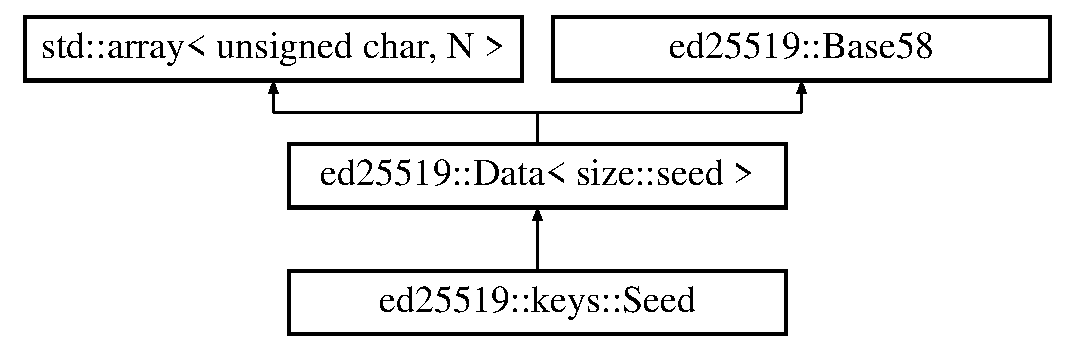
\includegraphics[height=3.000000cm]{classed25519_1_1keys_1_1_seed}
\end{center}
\end{figure}
\subsection*{Public Member Functions}
\begin{DoxyCompactItemize}
\item 
\mbox{\hyperlink{classed25519_1_1keys_1_1_seed_a81334bea98cdeb761ed600e8cec3dc8f}{Seed}} (const std\+::string \&phrase)
\item 
\mbox{\hyperlink{classed25519_1_1keys_1_1_seed_a63f29cc0551495dc2084b6f862ed75b5}{Seed}} ()
\end{DoxyCompactItemize}
\subsection*{Additional Inherited Members}


\subsection{Detailed Description}
\mbox{\hyperlink{classed25519_1_1keys_1_1_seed}{Seed}} data 

\subsection{Constructor \& Destructor Documentation}
\mbox{\Hypertarget{classed25519_1_1keys_1_1_seed_a81334bea98cdeb761ed600e8cec3dc8f}\label{classed25519_1_1keys_1_1_seed_a81334bea98cdeb761ed600e8cec3dc8f}} 
\index{ed25519\+::keys\+::\+Seed@{ed25519\+::keys\+::\+Seed}!Seed@{Seed}}
\index{Seed@{Seed}!ed25519\+::keys\+::\+Seed@{ed25519\+::keys\+::\+Seed}}
\subsubsection{\texorpdfstring{Seed()}{Seed()}\hspace{0.1cm}{\footnotesize\ttfamily [1/2]}}
{\footnotesize\ttfamily ed25519\+::keys\+::\+Seed\+::\+Seed (\begin{DoxyParamCaption}\item[{const std\+::string \&}]{phrase }\end{DoxyParamCaption})}

Create seed from secret phrase 
\begin{DoxyParams}{Parameters}
{\em phrase} & \\
\hline
\end{DoxyParams}
\mbox{\Hypertarget{classed25519_1_1keys_1_1_seed_a63f29cc0551495dc2084b6f862ed75b5}\label{classed25519_1_1keys_1_1_seed_a63f29cc0551495dc2084b6f862ed75b5}} 
\index{ed25519\+::keys\+::\+Seed@{ed25519\+::keys\+::\+Seed}!Seed@{Seed}}
\index{Seed@{Seed}!ed25519\+::keys\+::\+Seed@{ed25519\+::keys\+::\+Seed}}
\subsubsection{\texorpdfstring{Seed()}{Seed()}\hspace{0.1cm}{\footnotesize\ttfamily [2/2]}}
{\footnotesize\ttfamily ed25519\+::keys\+::\+Seed\+::\+Seed (\begin{DoxyParamCaption}{ }\end{DoxyParamCaption})}

Create random seed 

The documentation for this class was generated from the following file\+:\begin{DoxyCompactItemize}
\item 
/\+Users/denn/\+Development/\+Dehancer/\+Dehancer-\/\+Services/ed25519cpp/include/\mbox{\hyperlink{ed25519_8hpp}{ed25519.\+hpp}}\end{DoxyCompactItemize}

\hypertarget{classed25519_1_1_signature}{}\section{ed25519\+:\+:Signature Class Reference}
\label{classed25519_1_1_signature}\index{ed25519\+::\+Signature@{ed25519\+::\+Signature}}


{\ttfamily \#include $<$ed25519.\+hpp$>$}

Inheritance diagram for ed25519\+:\+:Signature\+:\begin{figure}[H]
\begin{center}
\leavevmode
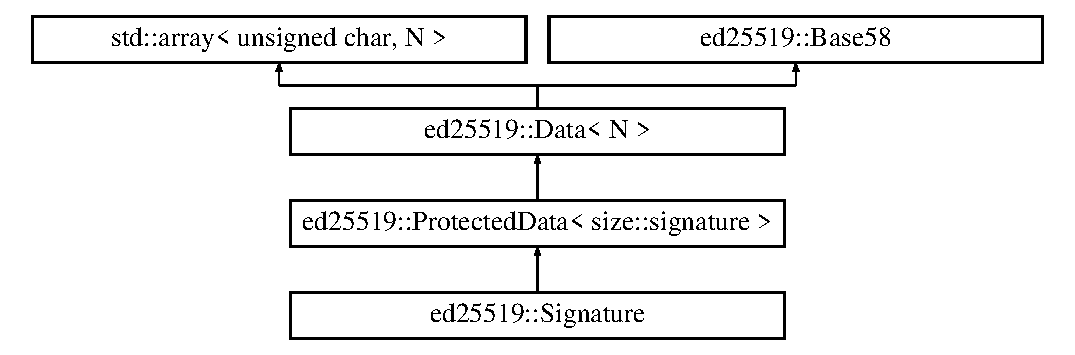
\includegraphics[height=3.000000cm]{classed25519_1_1_signature}
\end{center}
\end{figure}
\subsection*{Public Member Functions}
\begin{DoxyCompactItemize}
\item 
bool \mbox{\hyperlink{classed25519_1_1_signature_aca2ff60a3e305730cd62e7005b92cfef}{verify}} (const std\+::vector$<$ unsigned char $>$ \&message, const \mbox{\hyperlink{classed25519_1_1keys_1_1_public}{keys\+::\+Public}} \&key) const
\item 
bool \mbox{\hyperlink{classed25519_1_1_signature_a365b186127ea5150dd233c9c89ac4faf}{verify}} (const std\+::string \&message, const \mbox{\hyperlink{classed25519_1_1keys_1_1_public}{keys\+::\+Public}} \&key) const
\item 
bool \mbox{\hyperlink{classed25519_1_1_signature_a906ffca7764e7879438a9c60d96ff207}{verify}} (const \mbox{\hyperlink{structed25519_1_1_digest}{Digest}} \&digest, const \mbox{\hyperlink{classed25519_1_1keys_1_1_public}{keys\+::\+Public}} \&key) const
\end{DoxyCompactItemize}
\subsection*{Additional Inherited Members}


\subsection{Detailed Description}
Sigature hash class 

\subsection{Member Function Documentation}
\mbox{\Hypertarget{classed25519_1_1_signature_aca2ff60a3e305730cd62e7005b92cfef}\label{classed25519_1_1_signature_aca2ff60a3e305730cd62e7005b92cfef}} 
\index{ed25519\+::\+Signature@{ed25519\+::\+Signature}!verify@{verify}}
\index{verify@{verify}!ed25519\+::\+Signature@{ed25519\+::\+Signature}}
\subsubsection{\texorpdfstring{verify()}{verify()}\hspace{0.1cm}{\footnotesize\ttfamily [1/3]}}
{\footnotesize\ttfamily bool ed25519\+::\+Signature\+::verify (\begin{DoxyParamCaption}\item[{const std\+::vector$<$ unsigned char $>$ \&}]{message,  }\item[{const \mbox{\hyperlink{classed25519_1_1keys_1_1_public}{keys\+::\+Public}} \&}]{key }\end{DoxyParamCaption}) const}

\mbox{\Hypertarget{classed25519_1_1_signature_a365b186127ea5150dd233c9c89ac4faf}\label{classed25519_1_1_signature_a365b186127ea5150dd233c9c89ac4faf}} 
\index{ed25519\+::\+Signature@{ed25519\+::\+Signature}!verify@{verify}}
\index{verify@{verify}!ed25519\+::\+Signature@{ed25519\+::\+Signature}}
\subsubsection{\texorpdfstring{verify()}{verify()}\hspace{0.1cm}{\footnotesize\ttfamily [2/3]}}
{\footnotesize\ttfamily bool ed25519\+::\+Signature\+::verify (\begin{DoxyParamCaption}\item[{const std\+::string \&}]{message,  }\item[{const \mbox{\hyperlink{classed25519_1_1keys_1_1_public}{keys\+::\+Public}} \&}]{key }\end{DoxyParamCaption}) const}

\mbox{\Hypertarget{classed25519_1_1_signature_a906ffca7764e7879438a9c60d96ff207}\label{classed25519_1_1_signature_a906ffca7764e7879438a9c60d96ff207}} 
\index{ed25519\+::\+Signature@{ed25519\+::\+Signature}!verify@{verify}}
\index{verify@{verify}!ed25519\+::\+Signature@{ed25519\+::\+Signature}}
\subsubsection{\texorpdfstring{verify()}{verify()}\hspace{0.1cm}{\footnotesize\ttfamily [3/3]}}
{\footnotesize\ttfamily bool ed25519\+::\+Signature\+::verify (\begin{DoxyParamCaption}\item[{const \mbox{\hyperlink{structed25519_1_1_digest}{Digest}} \&}]{digest,  }\item[{const \mbox{\hyperlink{classed25519_1_1keys_1_1_public}{keys\+::\+Public}} \&}]{key }\end{DoxyParamCaption}) const}



The documentation for this class was generated from the following file\+:\begin{DoxyCompactItemize}
\item 
/\+Users/denn/\+Development/\+Dehancer/\+Dehancer-\/\+Services/ed25519cpp/include/\mbox{\hyperlink{ed25519_8hpp}{ed25519.\+hpp}}\end{DoxyCompactItemize}

\chapter{File Documentation}
\hypertarget{ed25519_8hpp}{}\section{/\+Users/denn/\+Development/\+Dehancer/\+Dehancer-\/\+Services/ed25519cpp/include/ed25519.hpp File Reference}
\label{ed25519_8hpp}\index{/\+Users/denn/\+Development/\+Dehancer/\+Dehancer-\/\+Services/ed25519cpp/include/ed25519.\+hpp@{/\+Users/denn/\+Development/\+Dehancer/\+Dehancer-\/\+Services/ed25519cpp/include/ed25519.\+hpp}}
{\ttfamily \#include $<$string$>$}\newline
{\ttfamily \#include $<$array$>$}\newline
{\ttfamily \#include $<$vector$>$}\newline
{\ttfamily \#include $<$sstream$>$}\newline
{\ttfamily \#include $<$functional$>$}\newline
{\ttfamily \#include $<$optional$>$}\newline
{\ttfamily \#include $<$cerrno$>$}\newline
{\ttfamily \#include $<$system\+\_\+error$>$}\newline
{\ttfamily \#include $<$variant$>$}\newline
\subsection*{Classes}
\begin{DoxyCompactItemize}
\item 
class \mbox{\hyperlink{classed25519_1_1error__category}{ed25519\+::error\+\_\+category}}
\item 
class \mbox{\hyperlink{classed25519_1_1_base58}{ed25519\+::\+Base58}}
\item 
class \mbox{\hyperlink{classed25519_1_1_data}{ed25519\+::\+Data$<$ N $>$}}
\item 
class \mbox{\hyperlink{classed25519_1_1_digest}{ed25519\+::\+Digest}}
\item 
struct \mbox{\hyperlink{structed25519_1_1_digest_1_1_calculator}{ed25519\+::\+Digest\+::\+Calculator}}
\item 
class \mbox{\hyperlink{classed25519_1_1_signature}{ed25519\+::\+Signature}}
\item 
class \mbox{\hyperlink{classed25519_1_1keys_1_1_seed}{ed25519\+::keys\+::\+Seed}}
\item 
class \mbox{\hyperlink{classed25519_1_1keys_1_1_public}{ed25519\+::keys\+::\+Public}}
\item 
class \mbox{\hyperlink{classed25519_1_1keys_1_1_private}{ed25519\+::keys\+::\+Private}}
\item 
class \mbox{\hyperlink{classed25519_1_1keys_1_1_pair}{ed25519\+::keys\+::\+Pair}}
\end{DoxyCompactItemize}
\subsection*{Namespaces}
\begin{DoxyCompactItemize}
\item 
 \mbox{\hyperlink{namespaceed25519}{ed25519}}
\item 
 \mbox{\hyperlink{namespaceed25519_1_1size}{ed25519\+::size}}
\item 
 \mbox{\hyperlink{namespaceed25519_1_1base58}{ed25519\+::base58}}
\item 
 \mbox{\hyperlink{namespaceed25519_1_1keys}{ed25519\+::keys}}
\end{DoxyCompactItemize}
\subsection*{Typedefs}
\begin{DoxyCompactItemize}
\item 
typedef std\+::function$<$ void(const std\+::error\+\_\+code \&code)$>$ \mbox{\hyperlink{namespaceed25519_a6ba572942b3c18591fc869d52a6b16e6}{ed25519\+::\+Error\+Handler}}
\end{DoxyCompactItemize}
\subsection*{Enumerations}
\begin{DoxyCompactItemize}
\item 
enum \mbox{\hyperlink{namespaceed25519_ac93d0b5156eaca22197055e902920bc4}{ed25519\+::error}} \+: int \{ \mbox{\hyperlink{namespaceed25519_ac93d0b5156eaca22197055e902920bc4a28729b5efcbf8605d4412dbb86c3963b}{ed25519\+::\+B\+A\+D\+F\+O\+R\+M\+AT}} = 1000, 
\mbox{\hyperlink{namespaceed25519_ac93d0b5156eaca22197055e902920bc4a4a6895889f9590d64f64599b968a48b0}{ed25519\+::\+U\+N\+E\+X\+P\+E\+C\+T\+E\+D\+\_\+\+S\+I\+ZE}} = 1001, 
\mbox{\hyperlink{namespaceed25519_ac93d0b5156eaca22197055e902920bc4ad16a8ea865652b7e7222111ab6f7ea36}{ed25519\+::\+E\+M\+P\+TY}} = 1002
 \}
\end{DoxyCompactItemize}
\subsection*{Functions}
\begin{DoxyCompactItemize}
\item 
uint\+\_\+least32\+\_\+t \mbox{\hyperlink{namespaceed25519_1_1base58_abd4c654a7eba31c01eef529e26a8c364}{ed25519\+::base58\+::crc32}} (unsigned char $\ast$buf, size\+\_\+t len)
\item 
std\+::string \mbox{\hyperlink{namespaceed25519_1_1base58_a857764be1561c5e59bab056d771f22a1}{ed25519\+::base58\+::encode}} (const std\+::vector$<$ unsigned char $>$ \&data)
\item 
bool \mbox{\hyperlink{namespaceed25519_1_1base58_ac8132589f5098b8de74d2dfb72f7bf65}{ed25519\+::base58\+::decode}} (const std\+::string \&str, std\+::vector$<$ unsigned char $>$ \&data)
\item 
bool \mbox{\hyperlink{namespaceed25519_1_1base58_a2b3ccbfdccfbcc3125de0070e5b37e67}{ed25519\+::base58\+::validate}} (const std\+::string \&str)
\item 
{\footnotesize template$<$size\+\_\+t N$>$ }\\bool \mbox{\hyperlink{namespaceed25519_1_1base58_a97f34fe5ffdd0da677a4cef6be3a5a60}{ed25519\+::base58\+::decode}} (const std\+::string \&base58, std\+::array$<$ unsigned char, N $>$ \&data, const Error\+Handler \&error=default\+\_\+error\+\_\+handler)
\item 
{\footnotesize template$<$size\+\_\+t N$>$ }\\std\+::string \mbox{\hyperlink{namespaceed25519_1_1base58_a9e1eded8fc634072114771f77046693a}{ed25519\+::base58\+::encode}} (const std\+::array$<$ unsigned char, N $>$ \&data)
\item 
const std\+::string \mbox{\hyperlink{namespaceed25519_a908061c627d853b0d7ca46bdf0082310}{ed25519\+::\+String\+Format}} (const char $\ast$format,...)
\end{DoxyCompactItemize}
\subsection*{Variables}
\begin{DoxyCompactItemize}
\item 
static auto \mbox{\hyperlink{namespaceed25519_a7c7bb6ed17541162959c33ed3e3b15fb}{ed25519\+::default\+\_\+error\+\_\+handler}} = \mbox{[}$\,$\mbox{]}(const std\+::error\+\_\+code \&code) \{\}
\item 
constexpr const size\+\_\+t \mbox{\hyperlink{namespaceed25519_1_1size_a0c20525cc9711076ec093177a8e36c25}{ed25519\+::size\+::hash}} = 32
\item 
constexpr const size\+\_\+t \mbox{\hyperlink{namespaceed25519_1_1size_ac853f864bb12792f88647a998c3c030f}{ed25519\+::size\+::double\+\_\+hash}} = hash$\ast$2
\item 
constexpr const size\+\_\+t \mbox{\hyperlink{namespaceed25519_1_1size_a8f8f1706b7e101ddc858ad26bdc010eb}{ed25519\+::size\+::public\+\_\+key}} = hash
\item 
constexpr const size\+\_\+t \mbox{\hyperlink{namespaceed25519_1_1size_ab3443d829236034a3824204b295de4d0}{ed25519\+::size\+::digest}} = hash
\item 
constexpr const size\+\_\+t \mbox{\hyperlink{namespaceed25519_1_1size_a25303466af2d7379e9ceb5955dd70b57}{ed25519\+::size\+::seed}} = hash
\item 
constexpr const size\+\_\+t \mbox{\hyperlink{namespaceed25519_1_1size_a2e21f8a4af0331d49145f1893a441eed}{ed25519\+::size\+::private\+\_\+key}} = double\+\_\+hash
\item 
constexpr const size\+\_\+t \mbox{\hyperlink{namespaceed25519_1_1size_adefacb85c80ee8d51c482044e6d79a26}{ed25519\+::size\+::signature}} = double\+\_\+hash
\end{DoxyCompactItemize}

\hypertarget{_r_e_a_d_m_e_8md}{}\section{/\+Users/denn/\+Development/\+Dehancer/\+Dehancer-\/\+Services/ed25519cpp/\+R\+E\+A\+D\+ME.md File Reference}
\label{_r_e_a_d_m_e_8md}\index{/Users/denn/Development/Dehancer/Dehancer-\/Services/ed25519cpp/README.md@{/Users/denn/Development/Dehancer/Dehancer-\/Services/ed25519cpp/README.md}}

%--- End generated contents ---

% Index
\backmatter
\newpage
\phantomsection
\clearemptydoublepage
\addcontentsline{toc}{chapter}{Index}
\printindex

\end{document}
